\section{tau42 scale factor extrapolation}
\label{tau42SF}

We extrapolate our $\Hww$ tagging scale factor, as in Equation~\ref{SF42}, 
 from hadronic W tagging scale factor, as in Equation~\ref{SF21},  plus an additional 
systematic uncertainty $\epsilon$, as in Equation~\ref{SF4221}. 


\begin{equation}
SF_{H} = \frac{\tau_{42}^{Data}}{\tau_{42}^{MC}}
\label{SF42}
\end{equation}

\begin{equation}
SF_{W} = \frac{\tau_{21}^{Data}}{\tau_{21}^{MC}}
\label{SF21}
\end{equation}


\begin{equation}
SF_{H} = SF_{W} + \epsilon
\label{SF4221}
\end{equation}


Derived from equation~\ref{SF4221}, we have equation~\ref{SFNew}.

\begin{equation}
SF_{H} = SF_{W} \Longleftrightarrow \frac{\tau_{42}^{Data}}{\tau_{42}^{MC}} = \frac{\tau_{21}^{Data}}{\tau_{21}^{MC}} \Longleftrightarrow \frac{\tau_{42}^{Data}}{\tau_{21}^{Data}} = \frac{\tau_{42}^{MC}}{\tau_{21}^{MC}}
\label{SFNew}
\end{equation}

We validate equation~\ref{SFNew} by comparing the $\frac{\tau_{42}}{\tau_{21}}$ in data and 
\PYTHIA and \HERWIG QCD MC, as shown in Figure~\ref{fig:tau4221samejet}, ~\ref{fig:tau4221samejetH}
 and ~\ref{fig:tau4221samejetL}. In this plot
MC shows resonably good agreement with data. 
 
\begin{figure}[htb]
\begin{center}
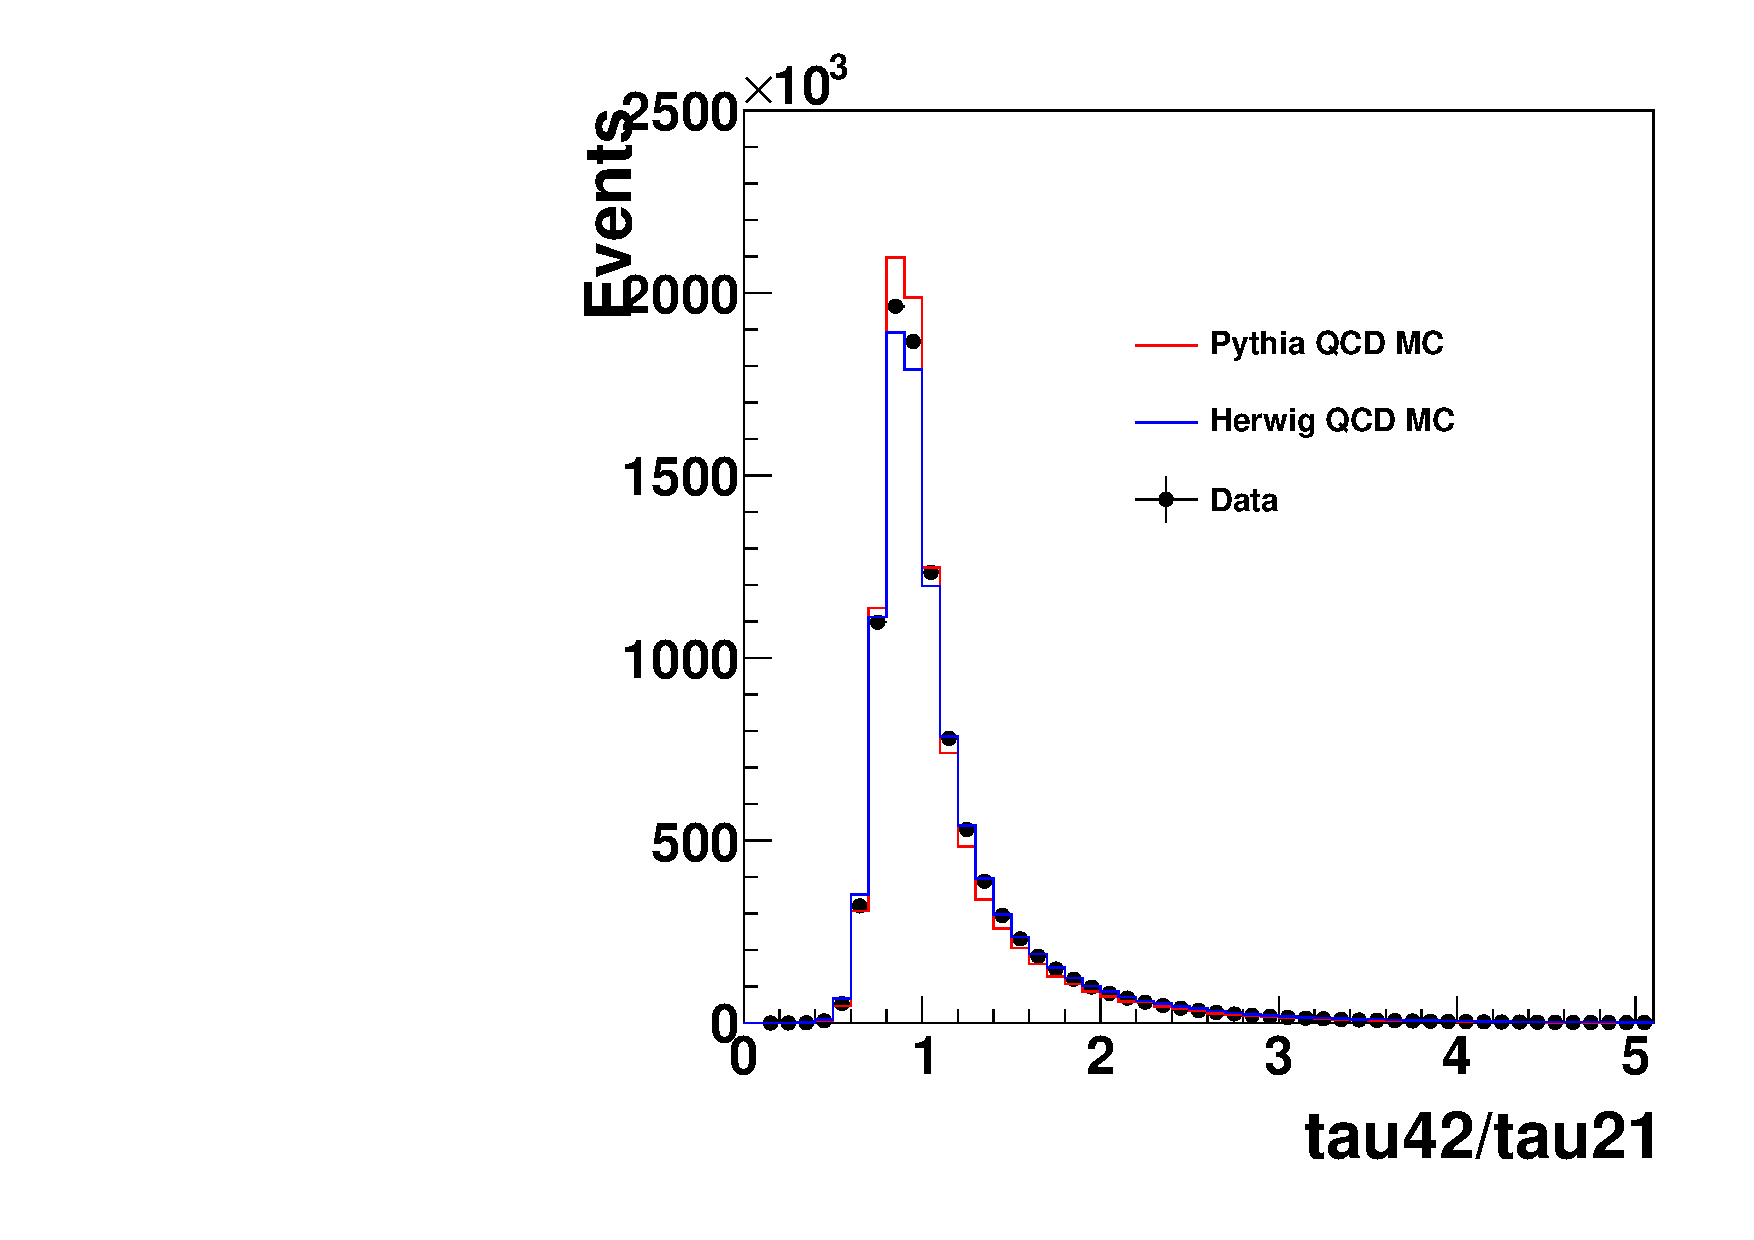
\includegraphics[width=0.49\textwidth,angle=0]{figs/SFExtra/SFSameJetRatioPlot.pdf}
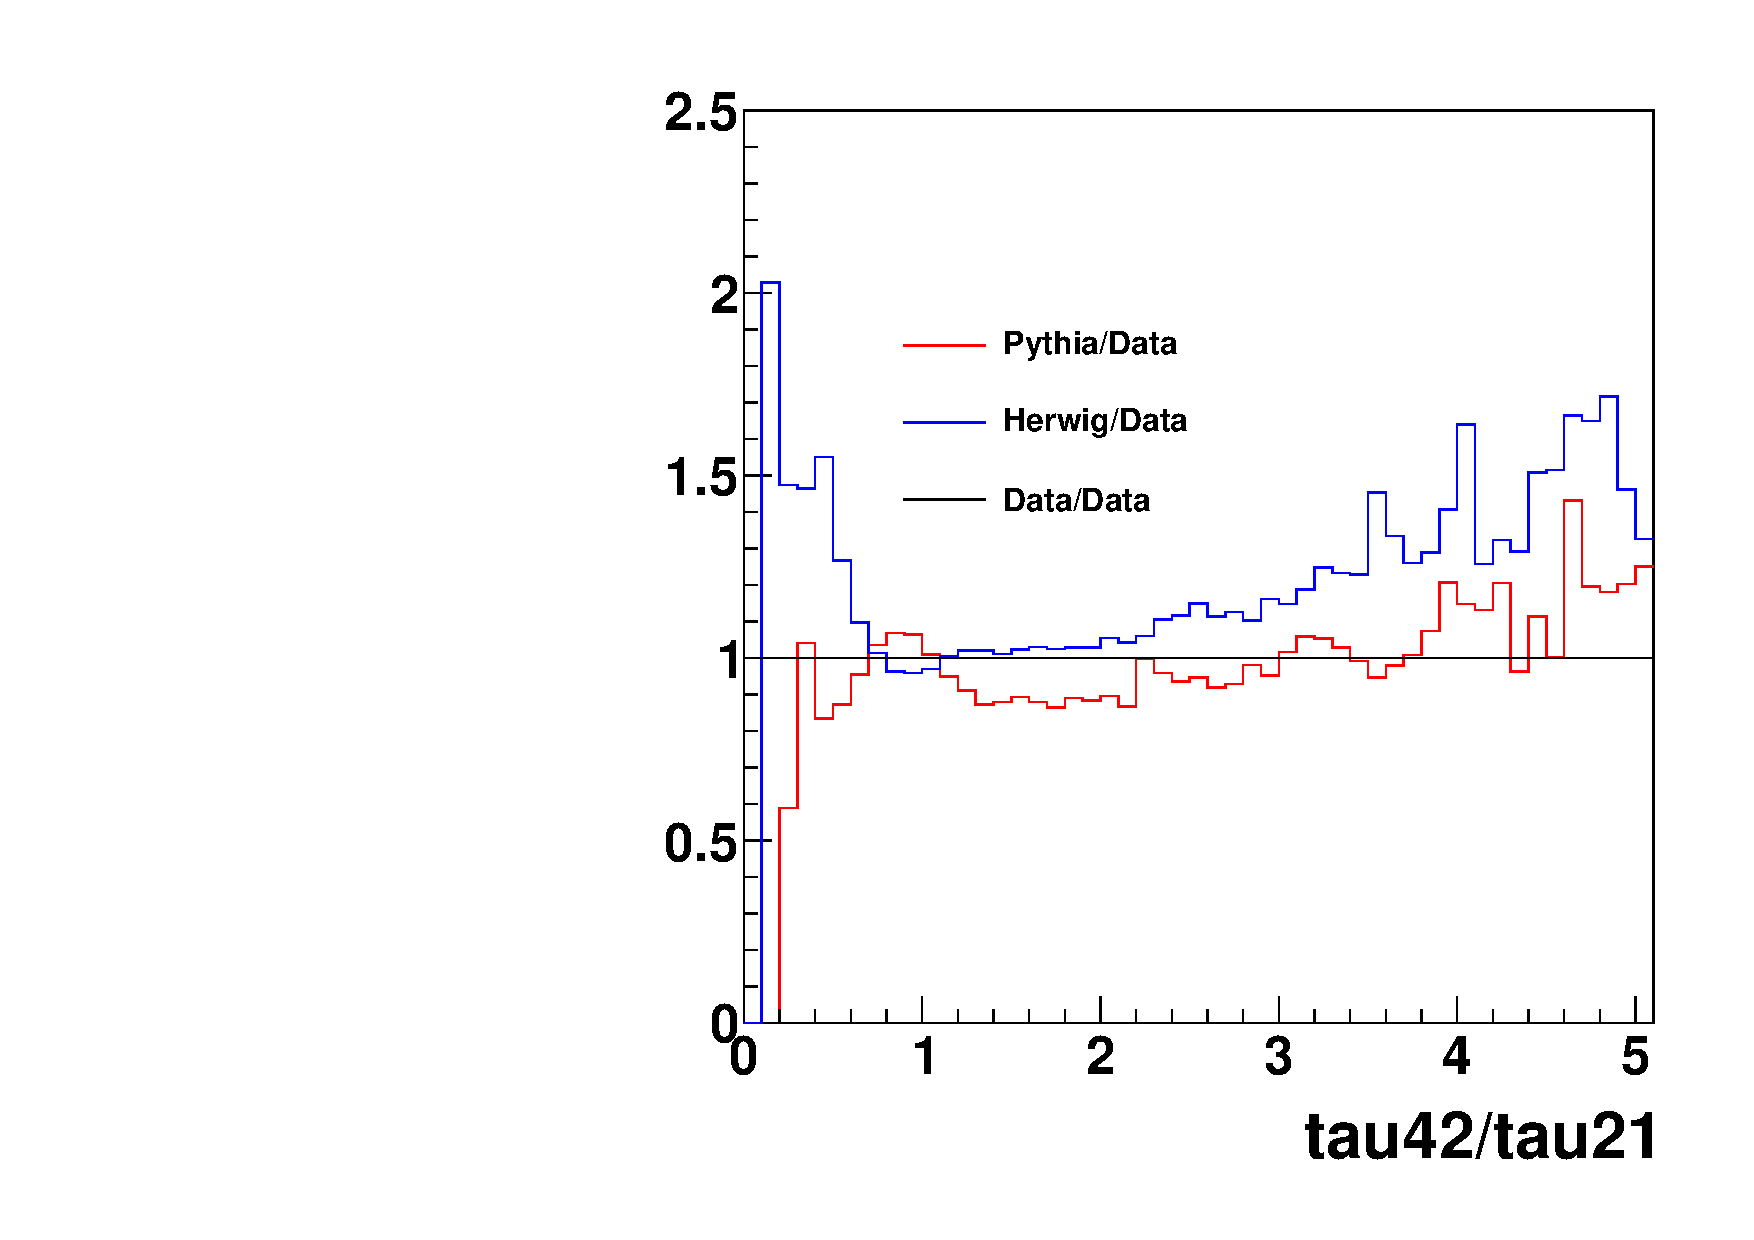
\includegraphics[width=0.49\textwidth,angle=0]{figs/SFExtra/SFRatioRatioPlot.pdf}
%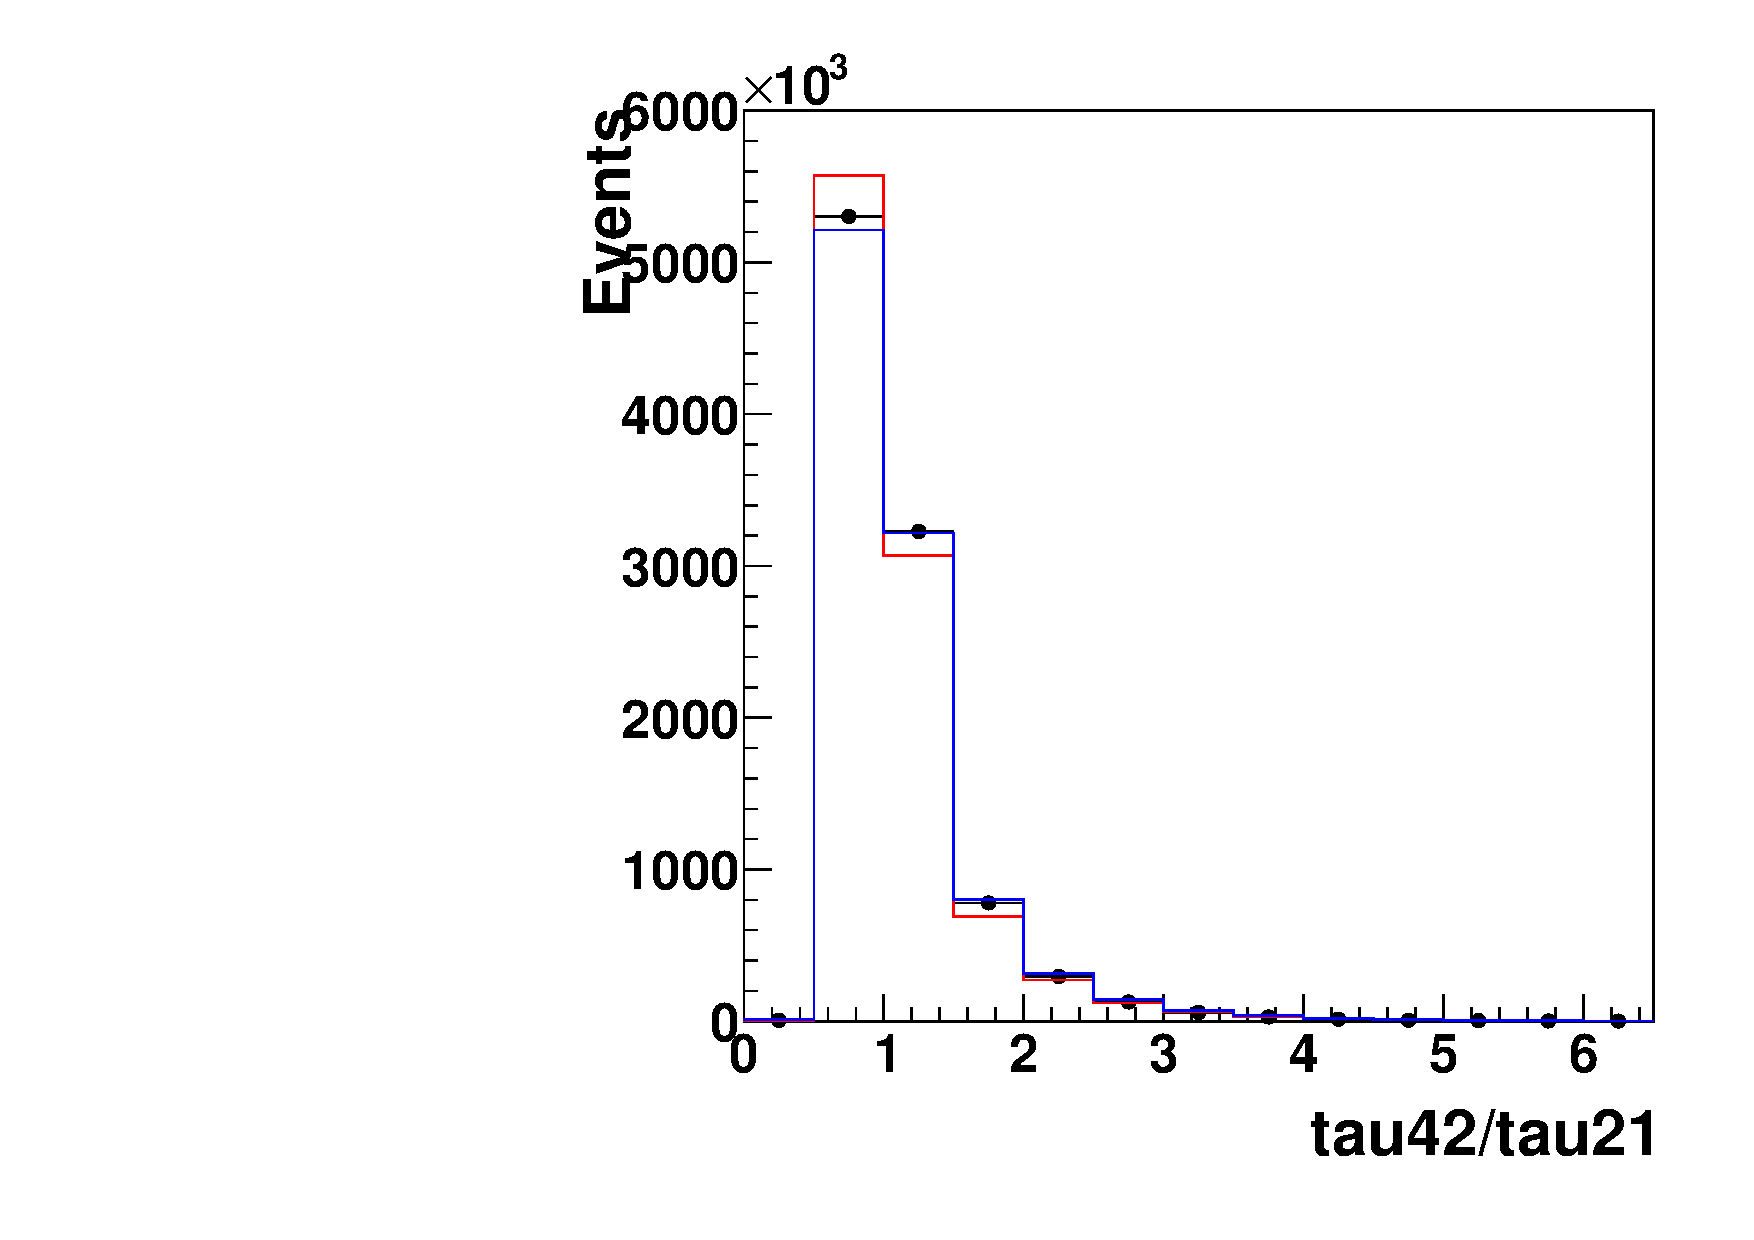
\includegraphics[width=0.49\textwidth,angle=0]{figs/SFExtra/SFSameJet.pdf}
%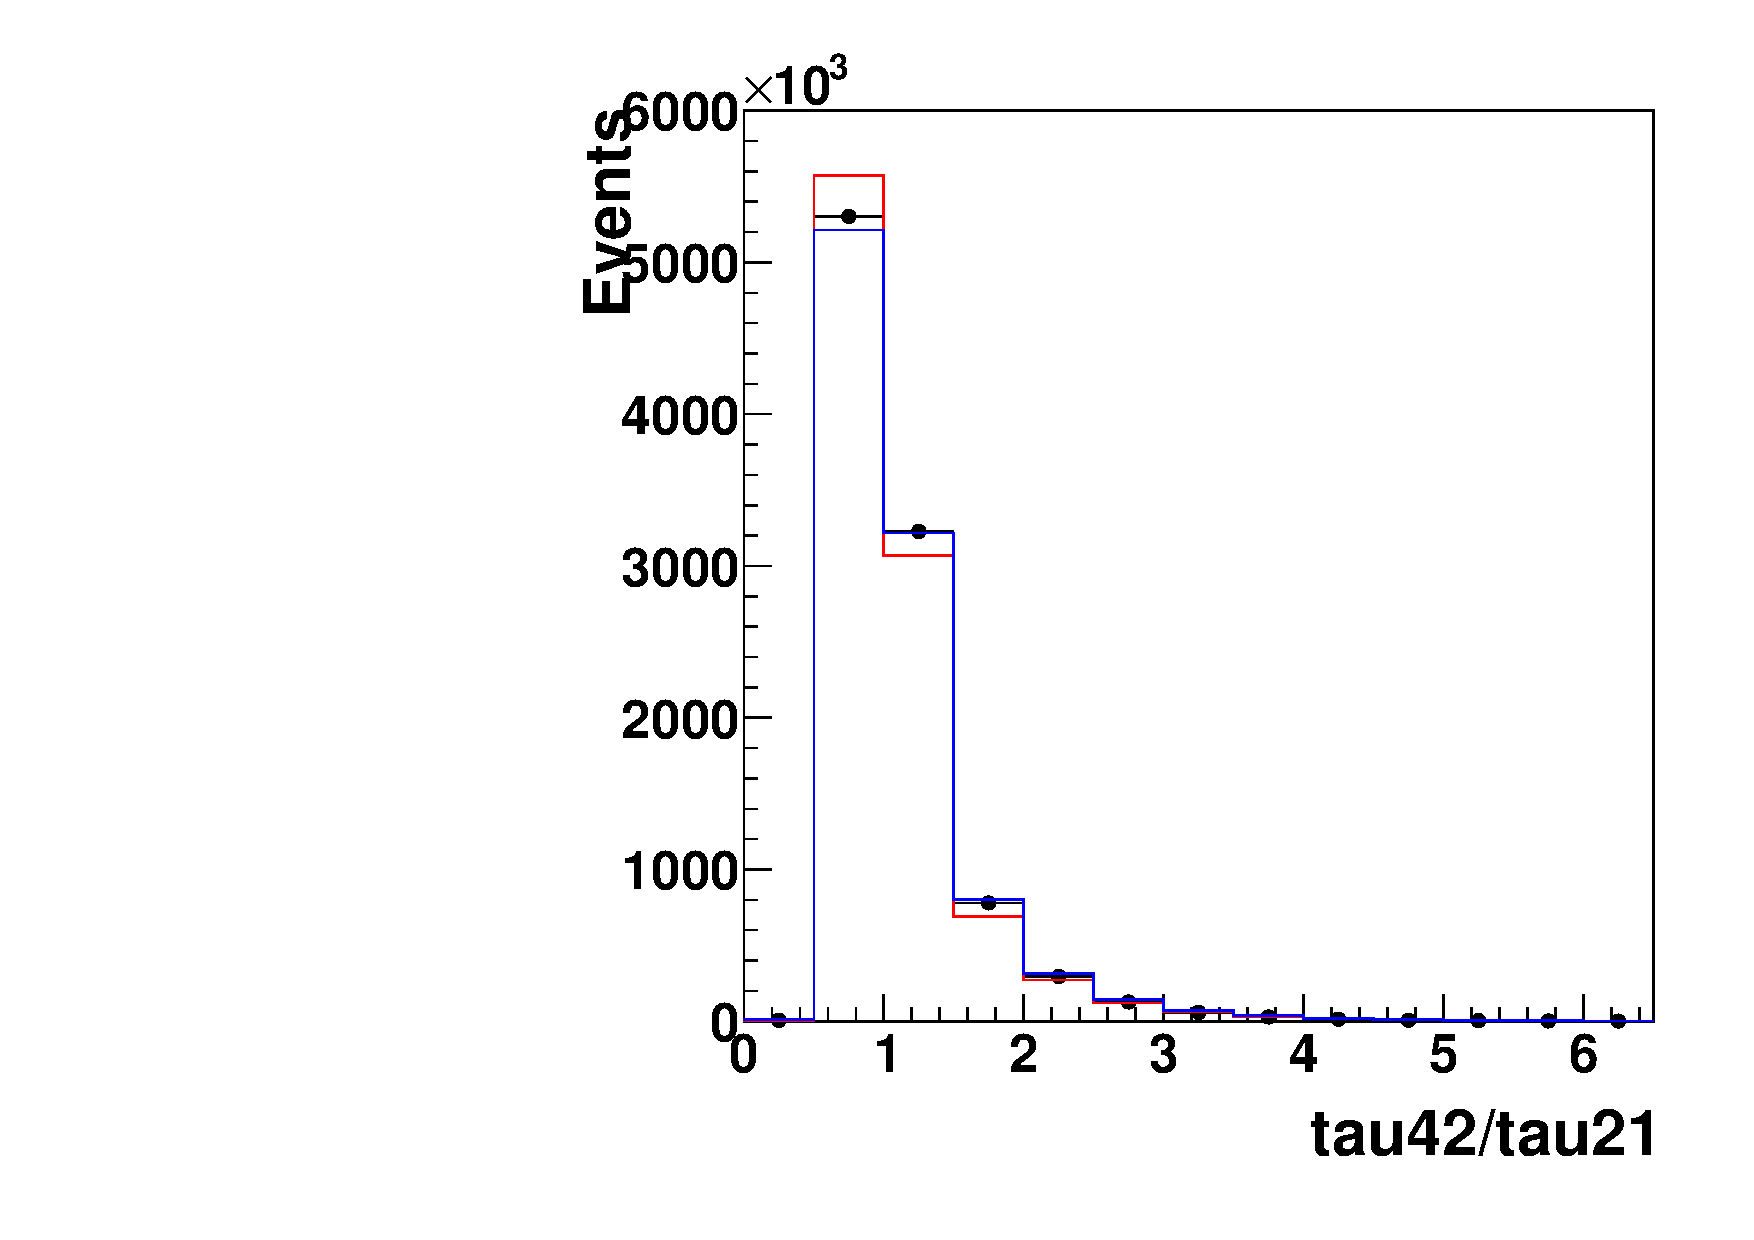
\includegraphics[width=0.49\textwidth,angle=0]{figs/SFExtra/SFSameJet.pdf}
\end{center}
\caption{
$\frac{\tau_{42}}{\tau_{21}}$ in data (black) compared to \PYTHIA QCD MC (red), and 
\HERWIG QCD MC (blue). Left hand plot is logY scale. Plot on the right hand is corresponding 
ratio plot of left hand.  
}
\label{fig:tau4221samejet}
\end{figure}

\begin{figure}[htb]
\begin{center}
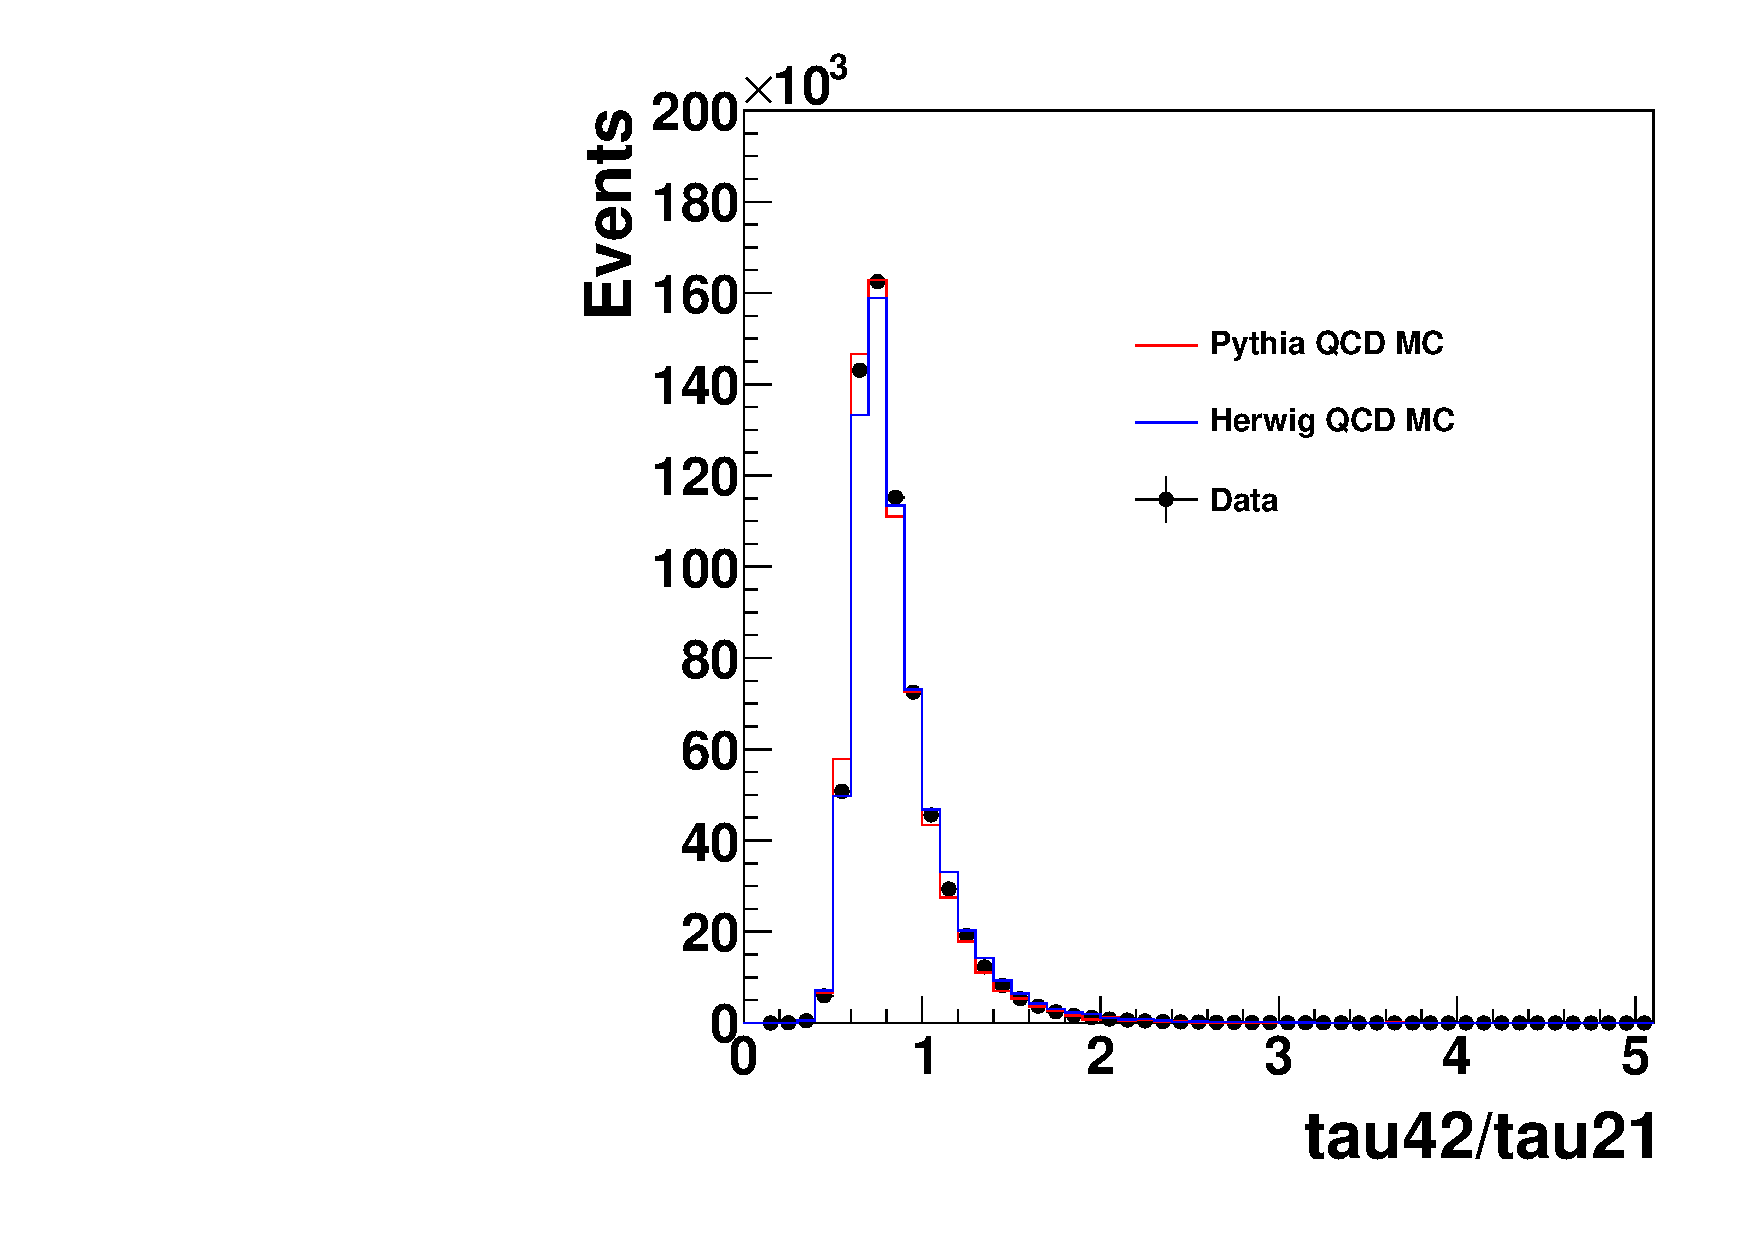
\includegraphics[width=0.49\textwidth,angle=0]{figs/SFExtra/SFSameJetRatioPlot55H.pdf}
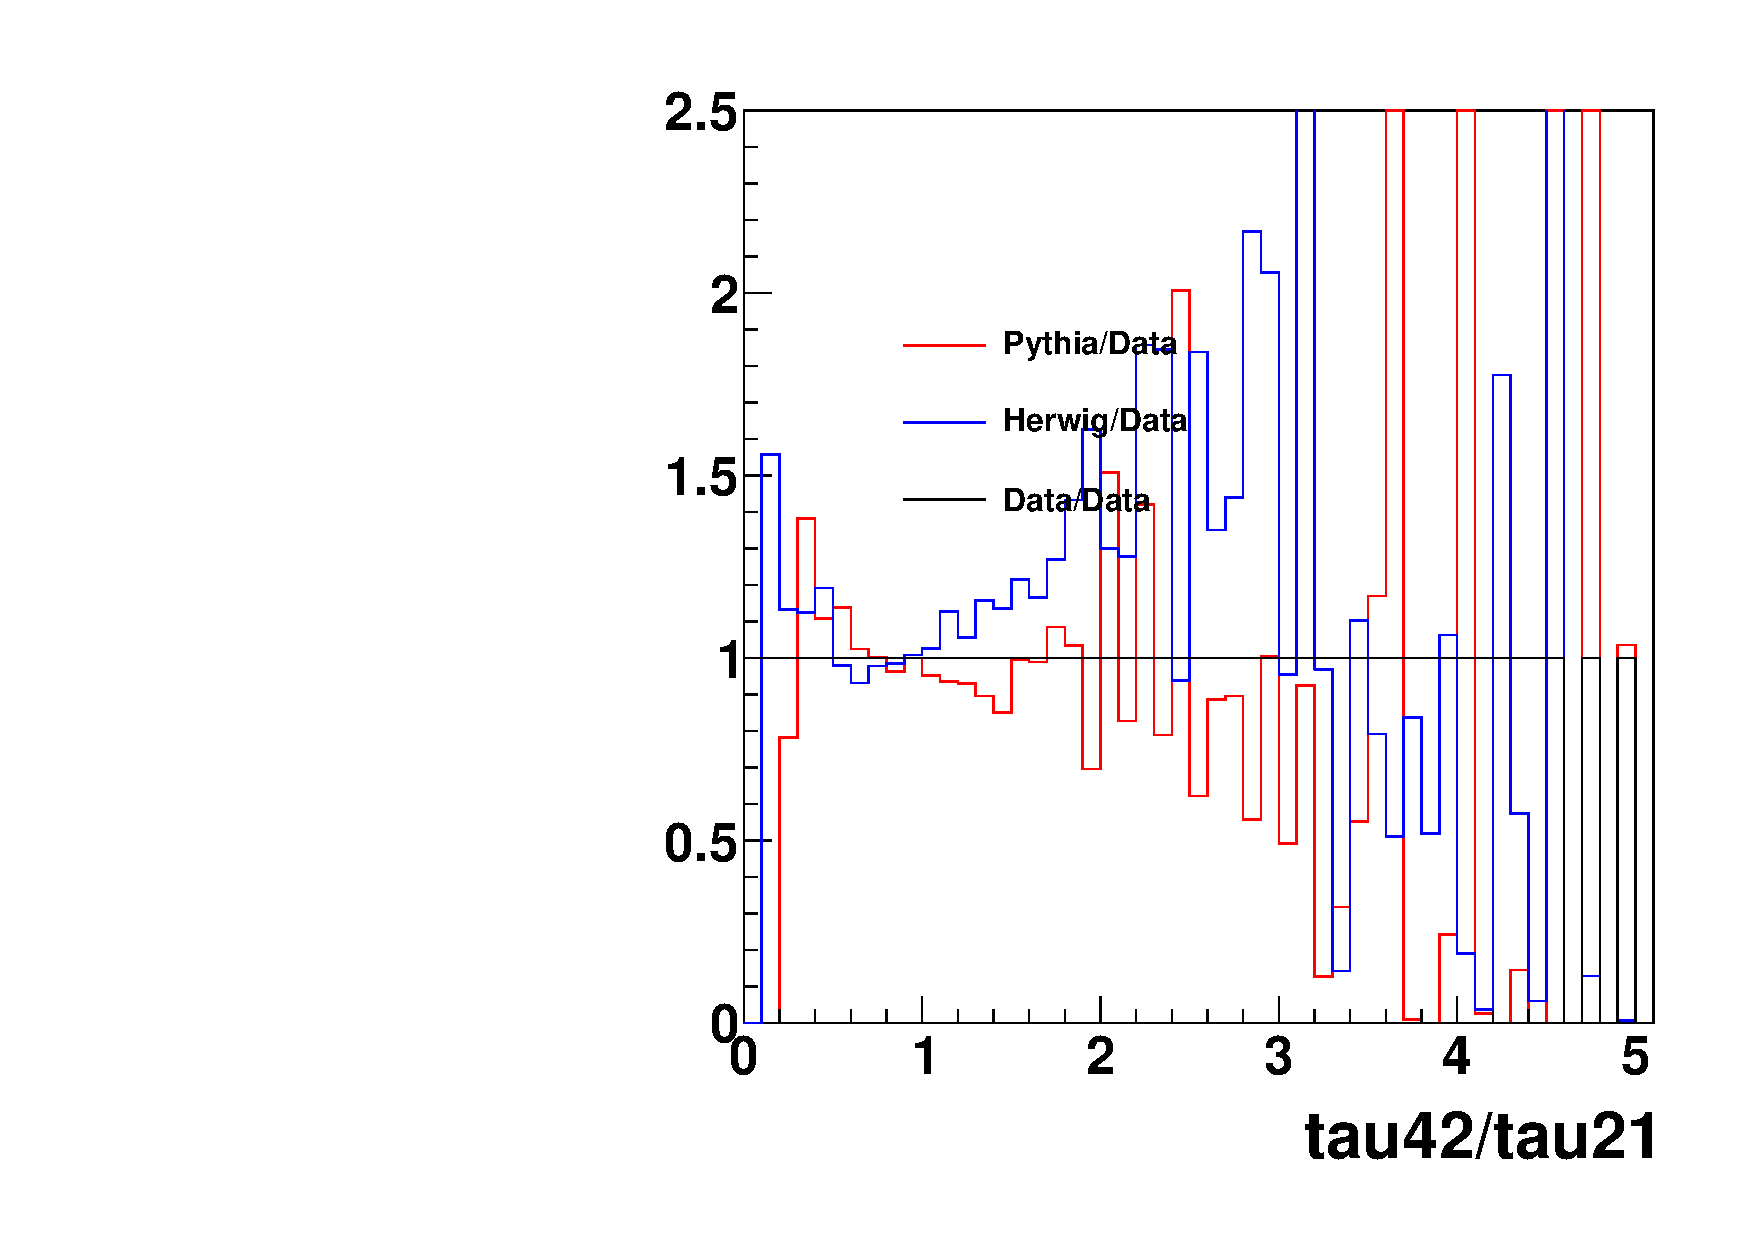
\includegraphics[width=0.49\textwidth,angle=0]{figs/SFExtra/SFRatioRatioPlot55H.pdf}
%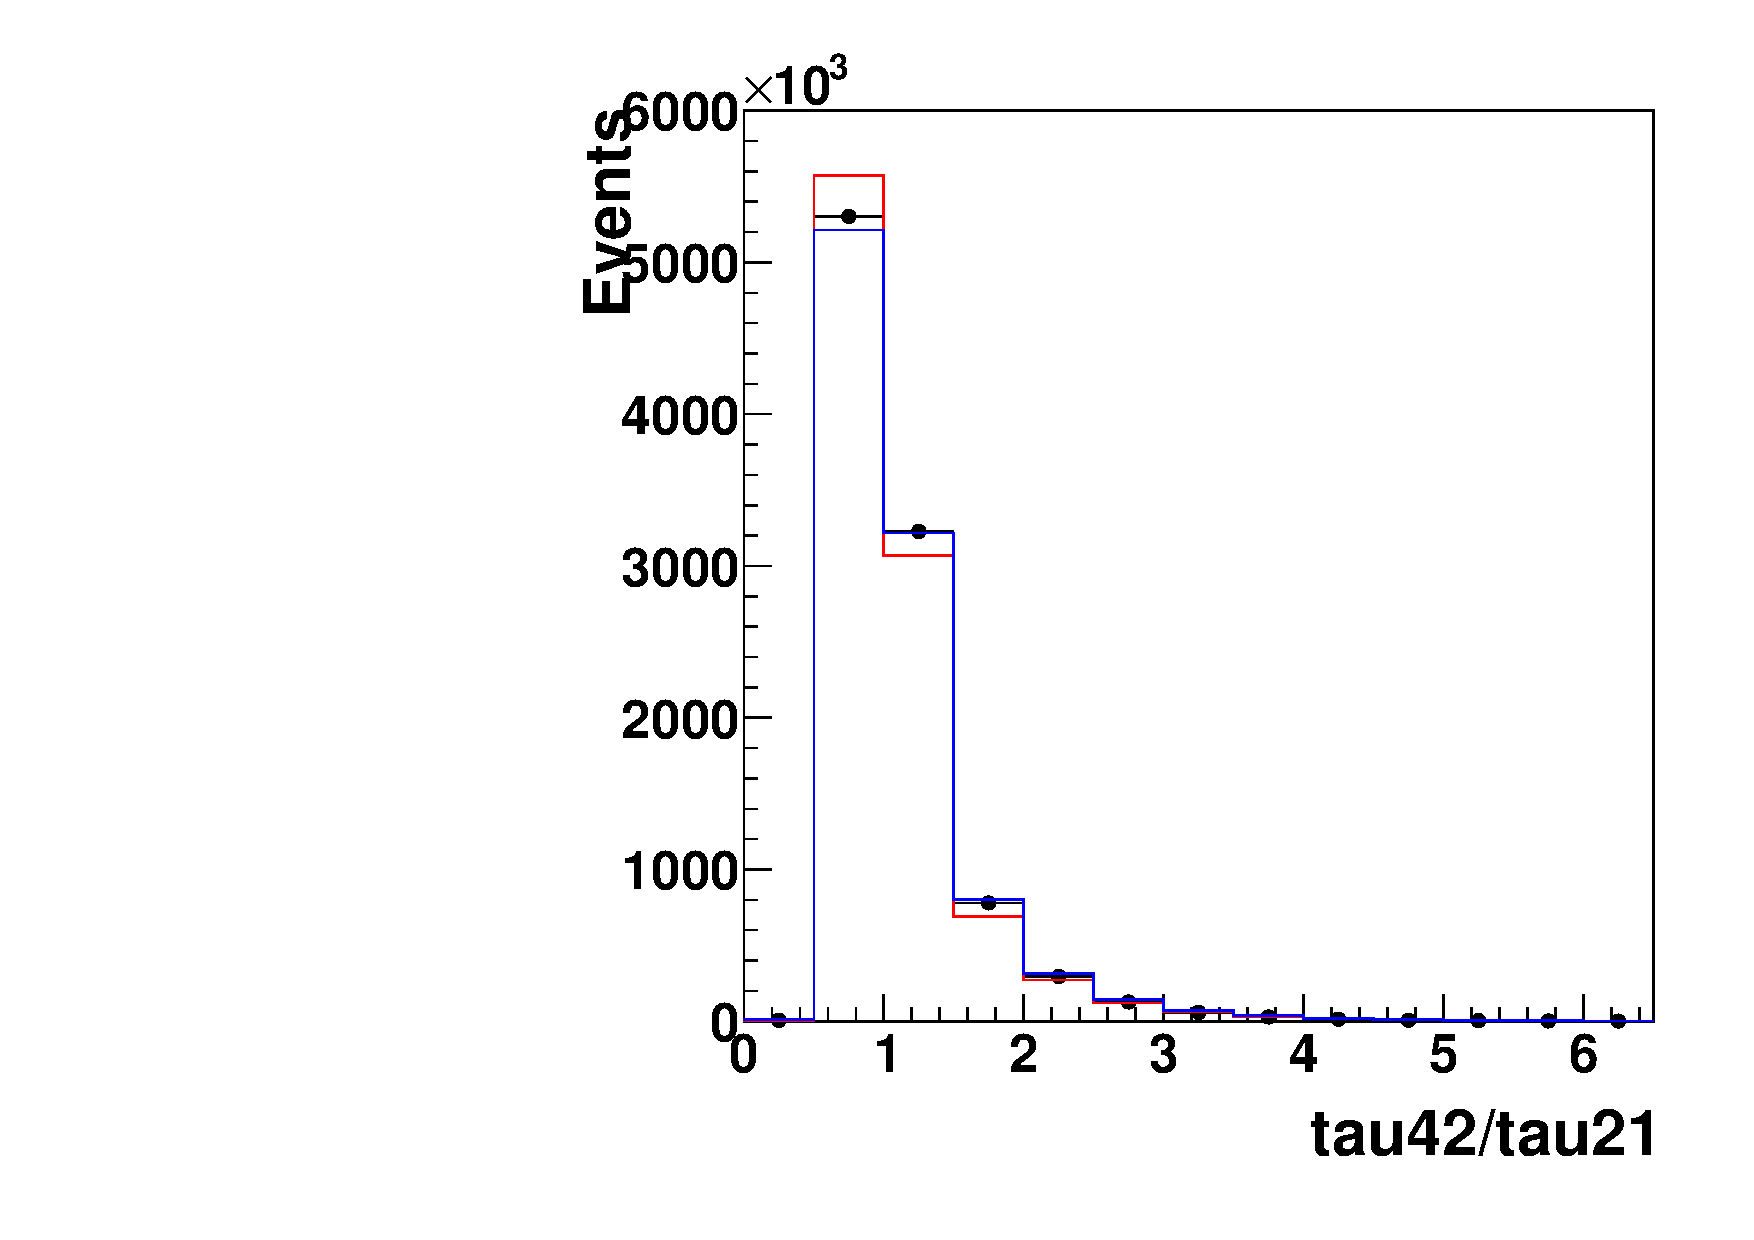
\includegraphics[width=0.49\textwidth,angle=0]{figs/SFExtra/SFSameJet.pdf}
%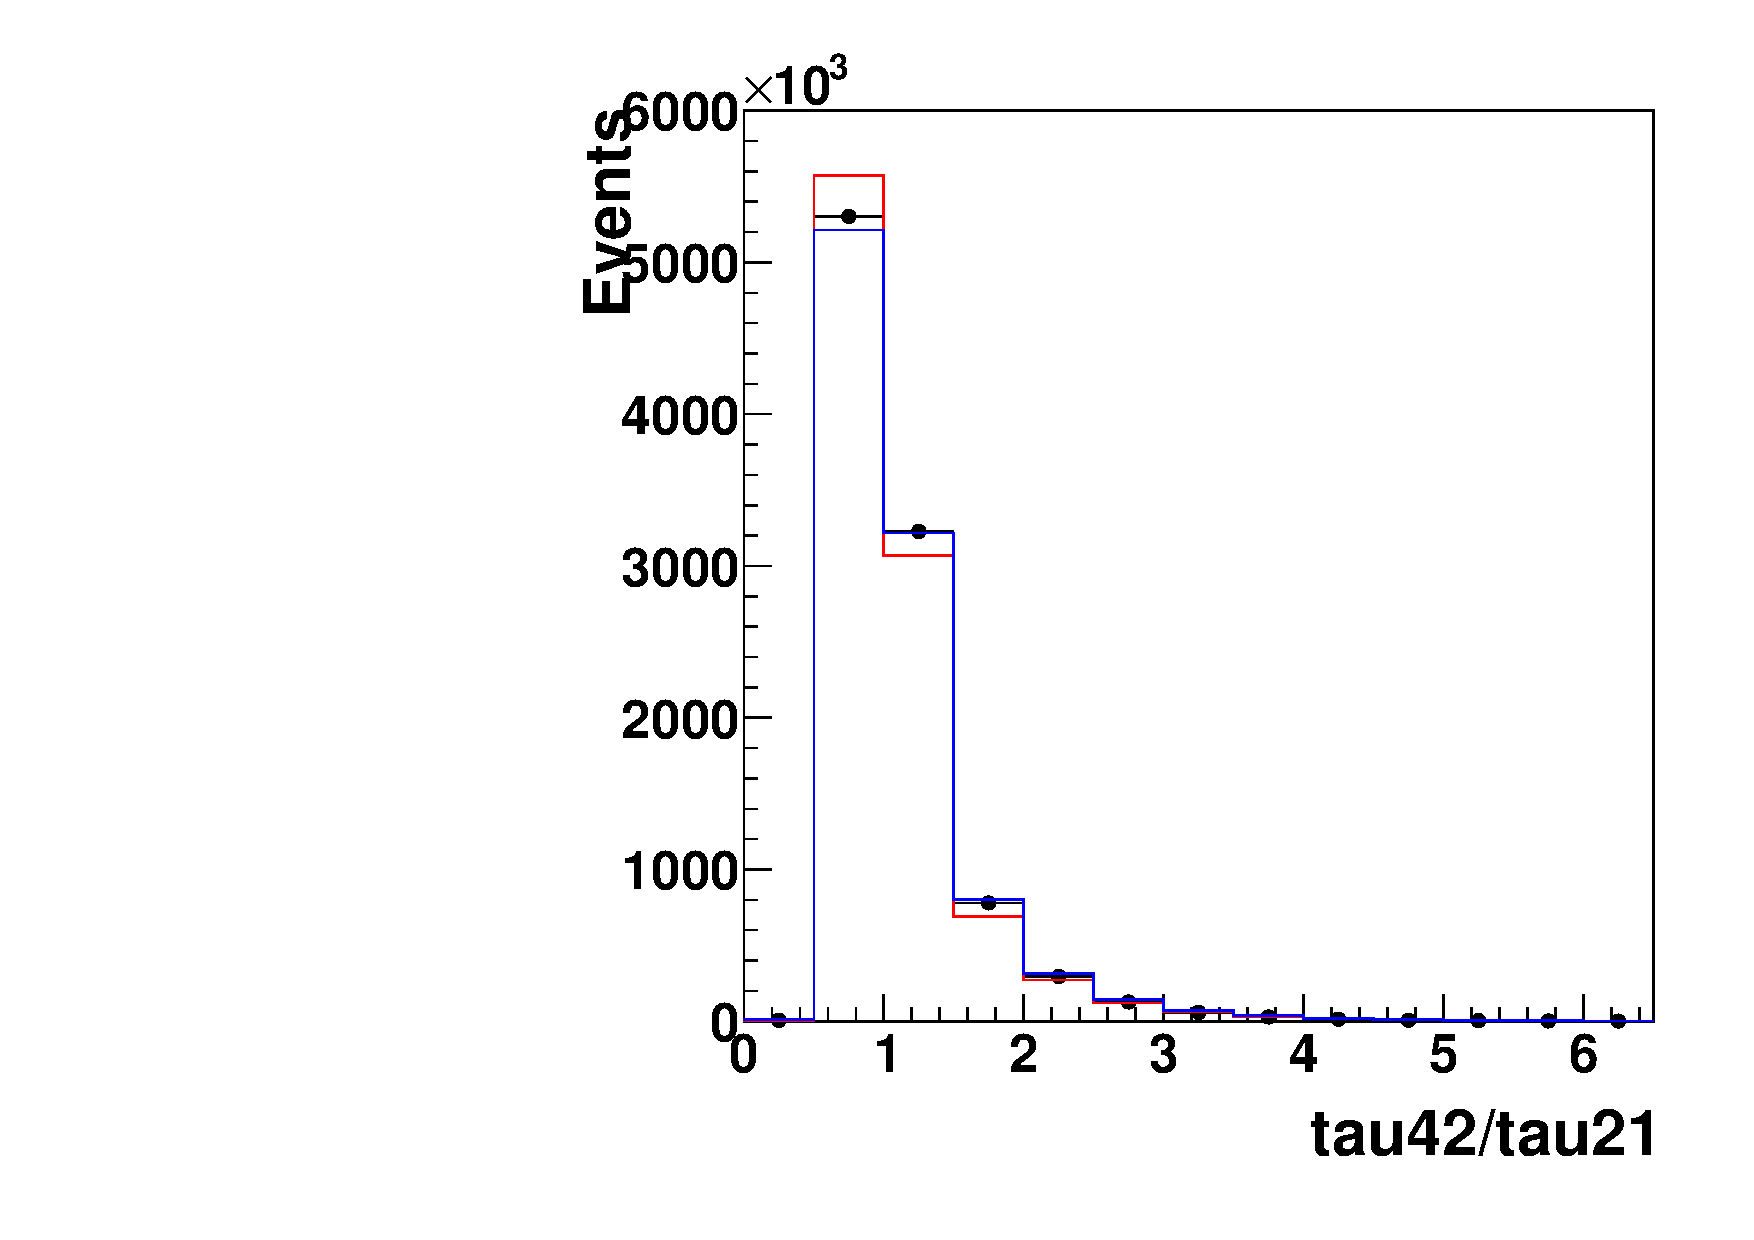
\includegraphics[width=0.49\textwidth,angle=0]{figs/SFExtra/SFSameJet.pdf}
\end{center}
\caption{
$\frac{\tau_{42}}{\tau_{21}}$ in data (black) compared to \PYTHIA QCD MC (red), and 
\HERWIG QCD MC (blue). Region of $\tau_{42} < 0.55$ is shown. 
Left hand plot is logY scale. Plot on the right hand is corresponding 
ratio plot of left hand.  
}
\label{fig:tau4221samejetH}
\end{figure}

\begin{figure}[htb]
\begin{center}
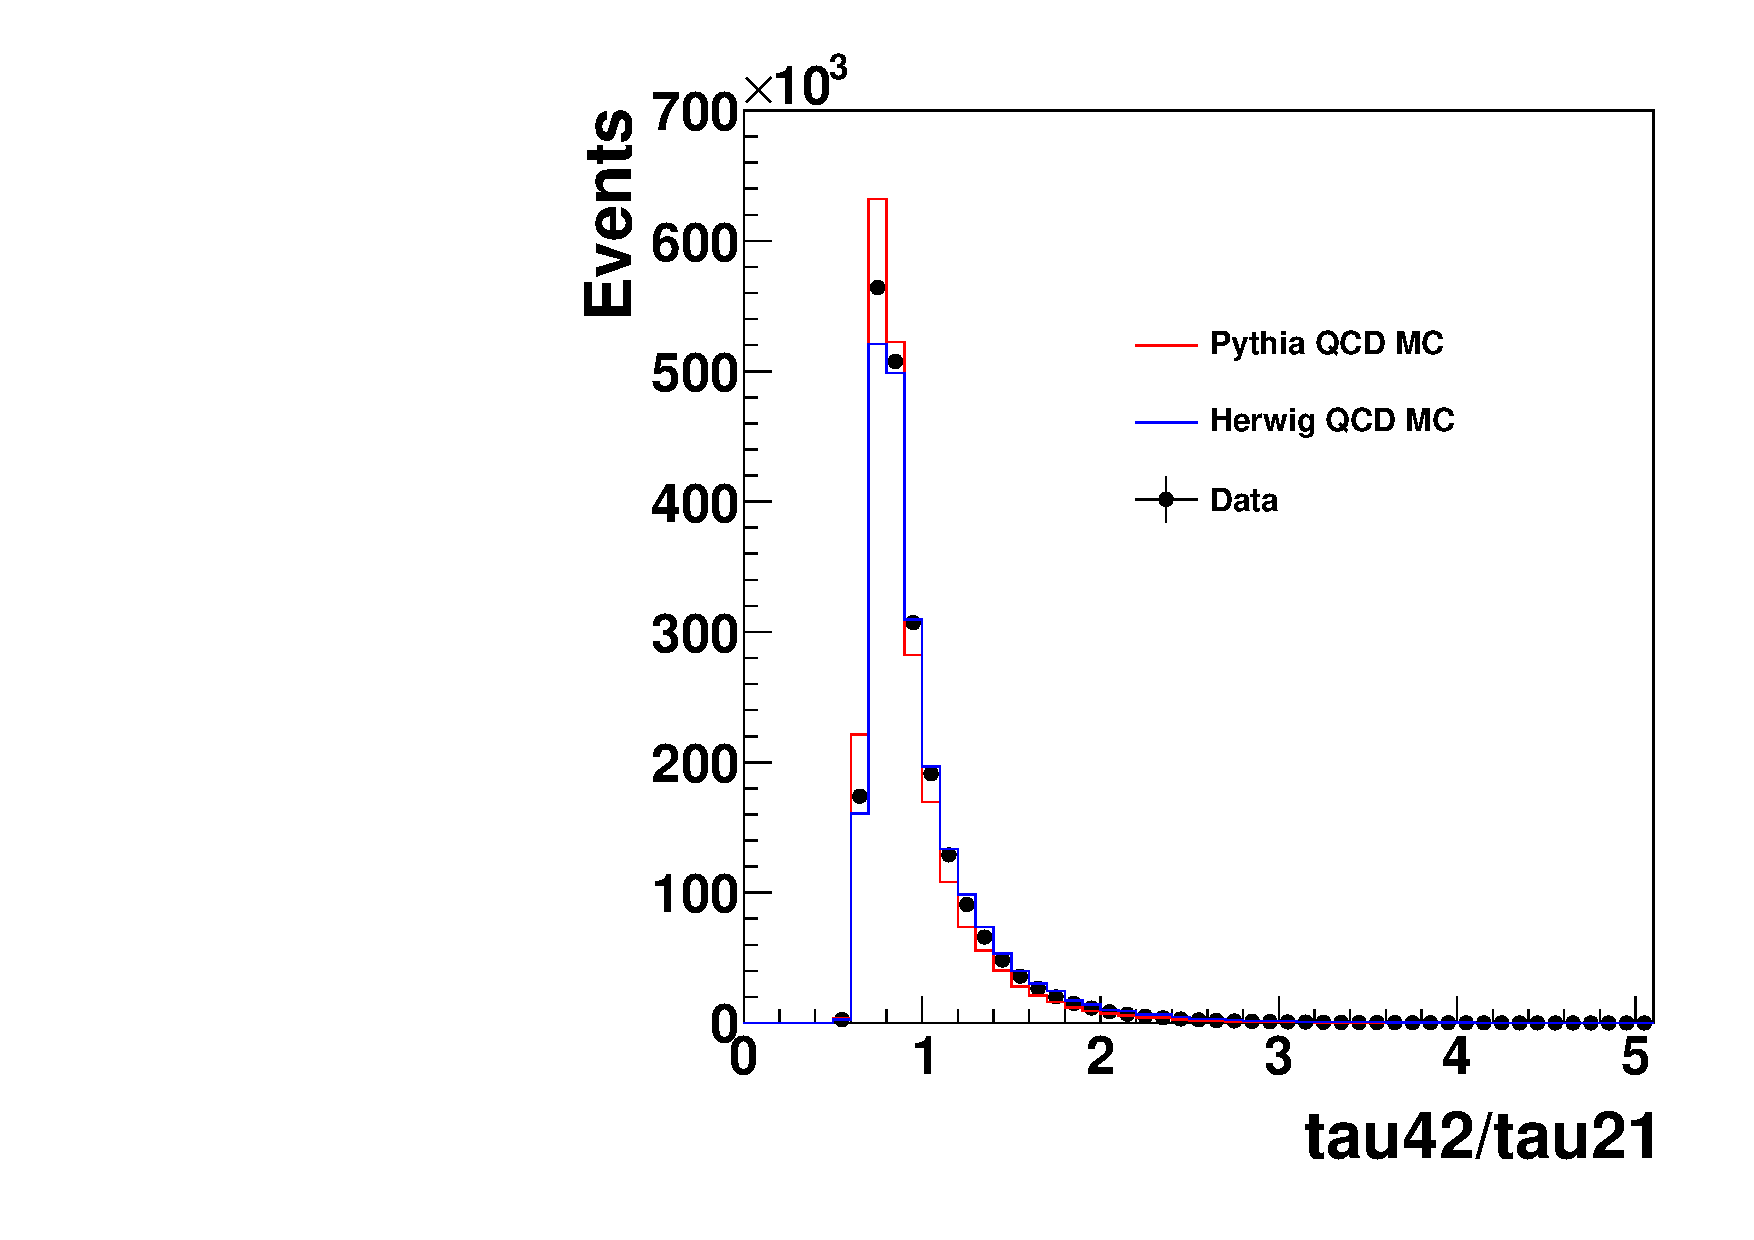
\includegraphics[width=0.49\textwidth,angle=0]{figs/SFExtra/SFSameJetRatioPlot55L.pdf}
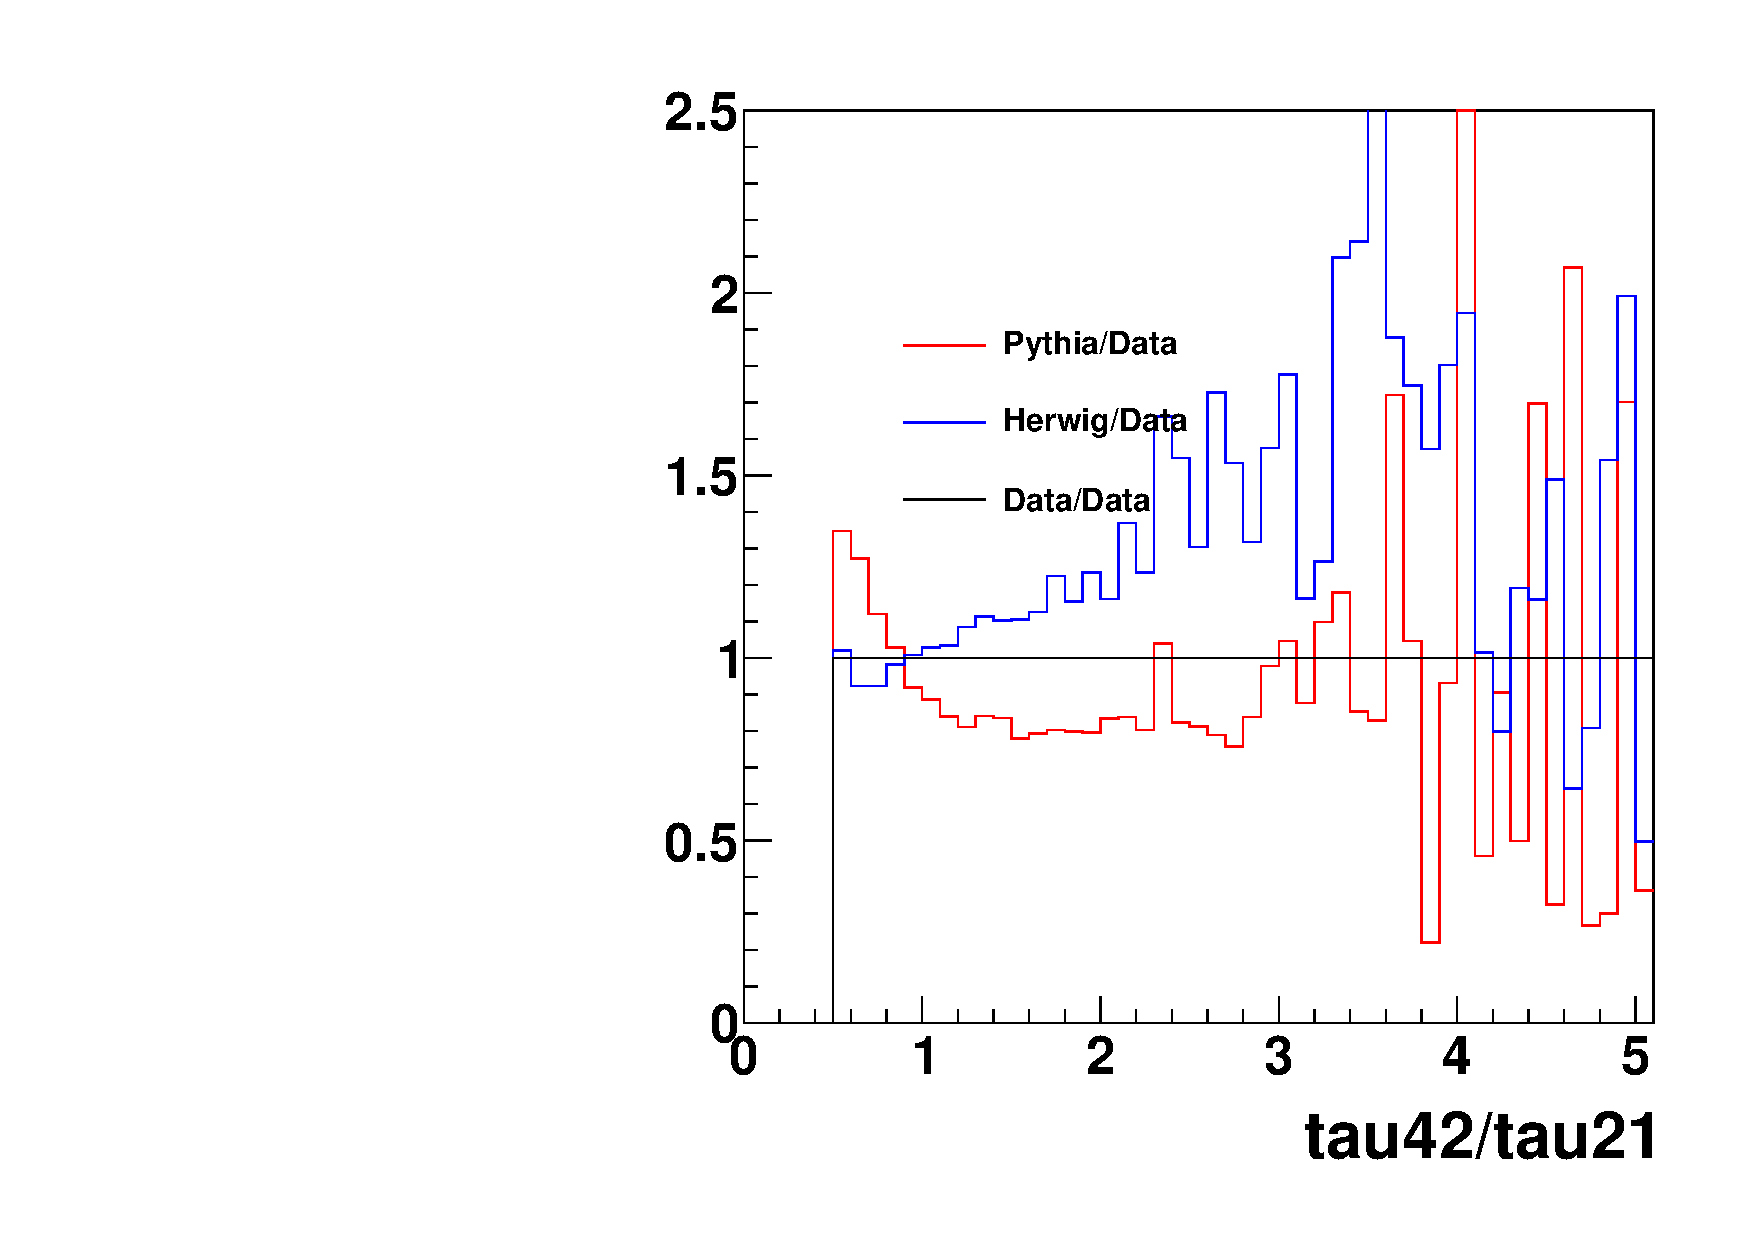
\includegraphics[width=0.49\textwidth,angle=0]{figs/SFExtra/SFRatioRatioPlot55L.pdf}
%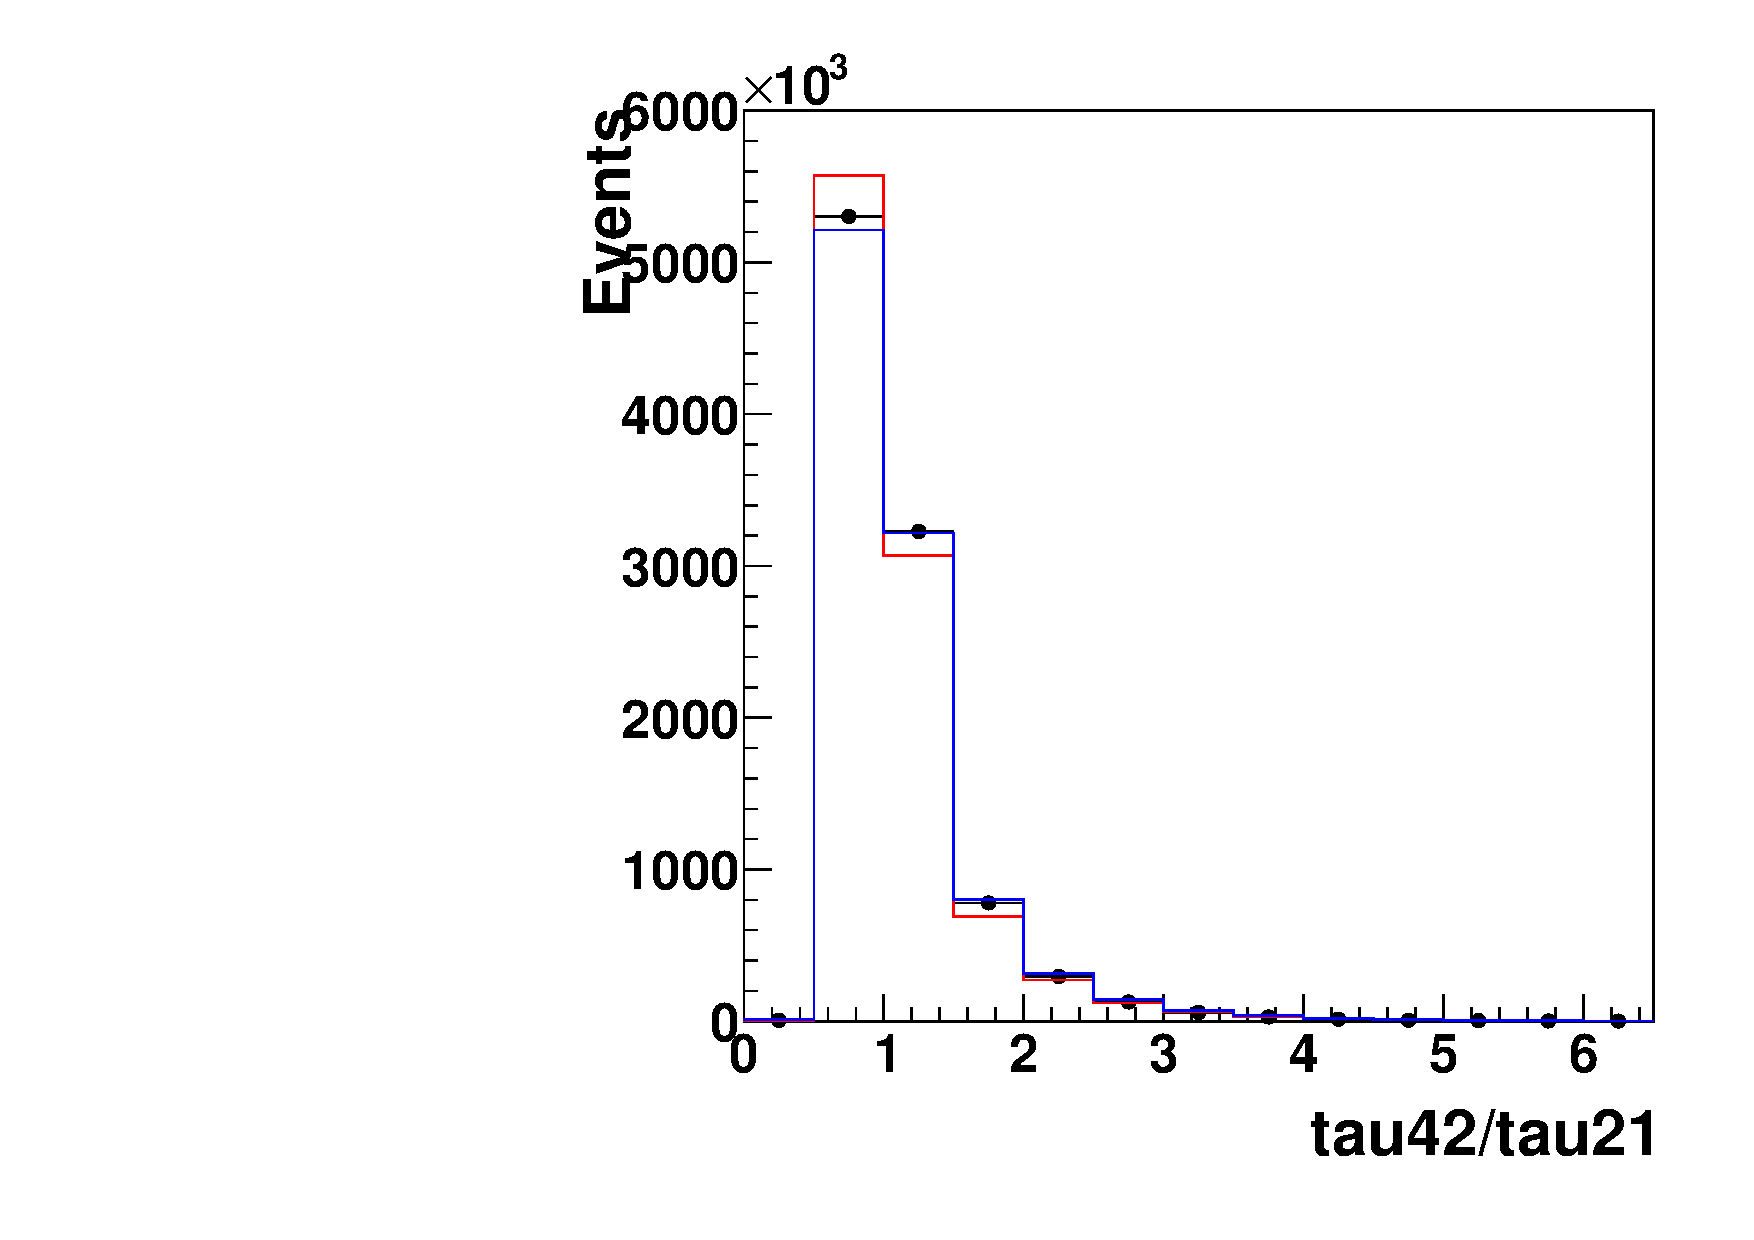
\includegraphics[width=0.49\textwidth,angle=0]{figs/SFExtra/SFSameJet.pdf}
%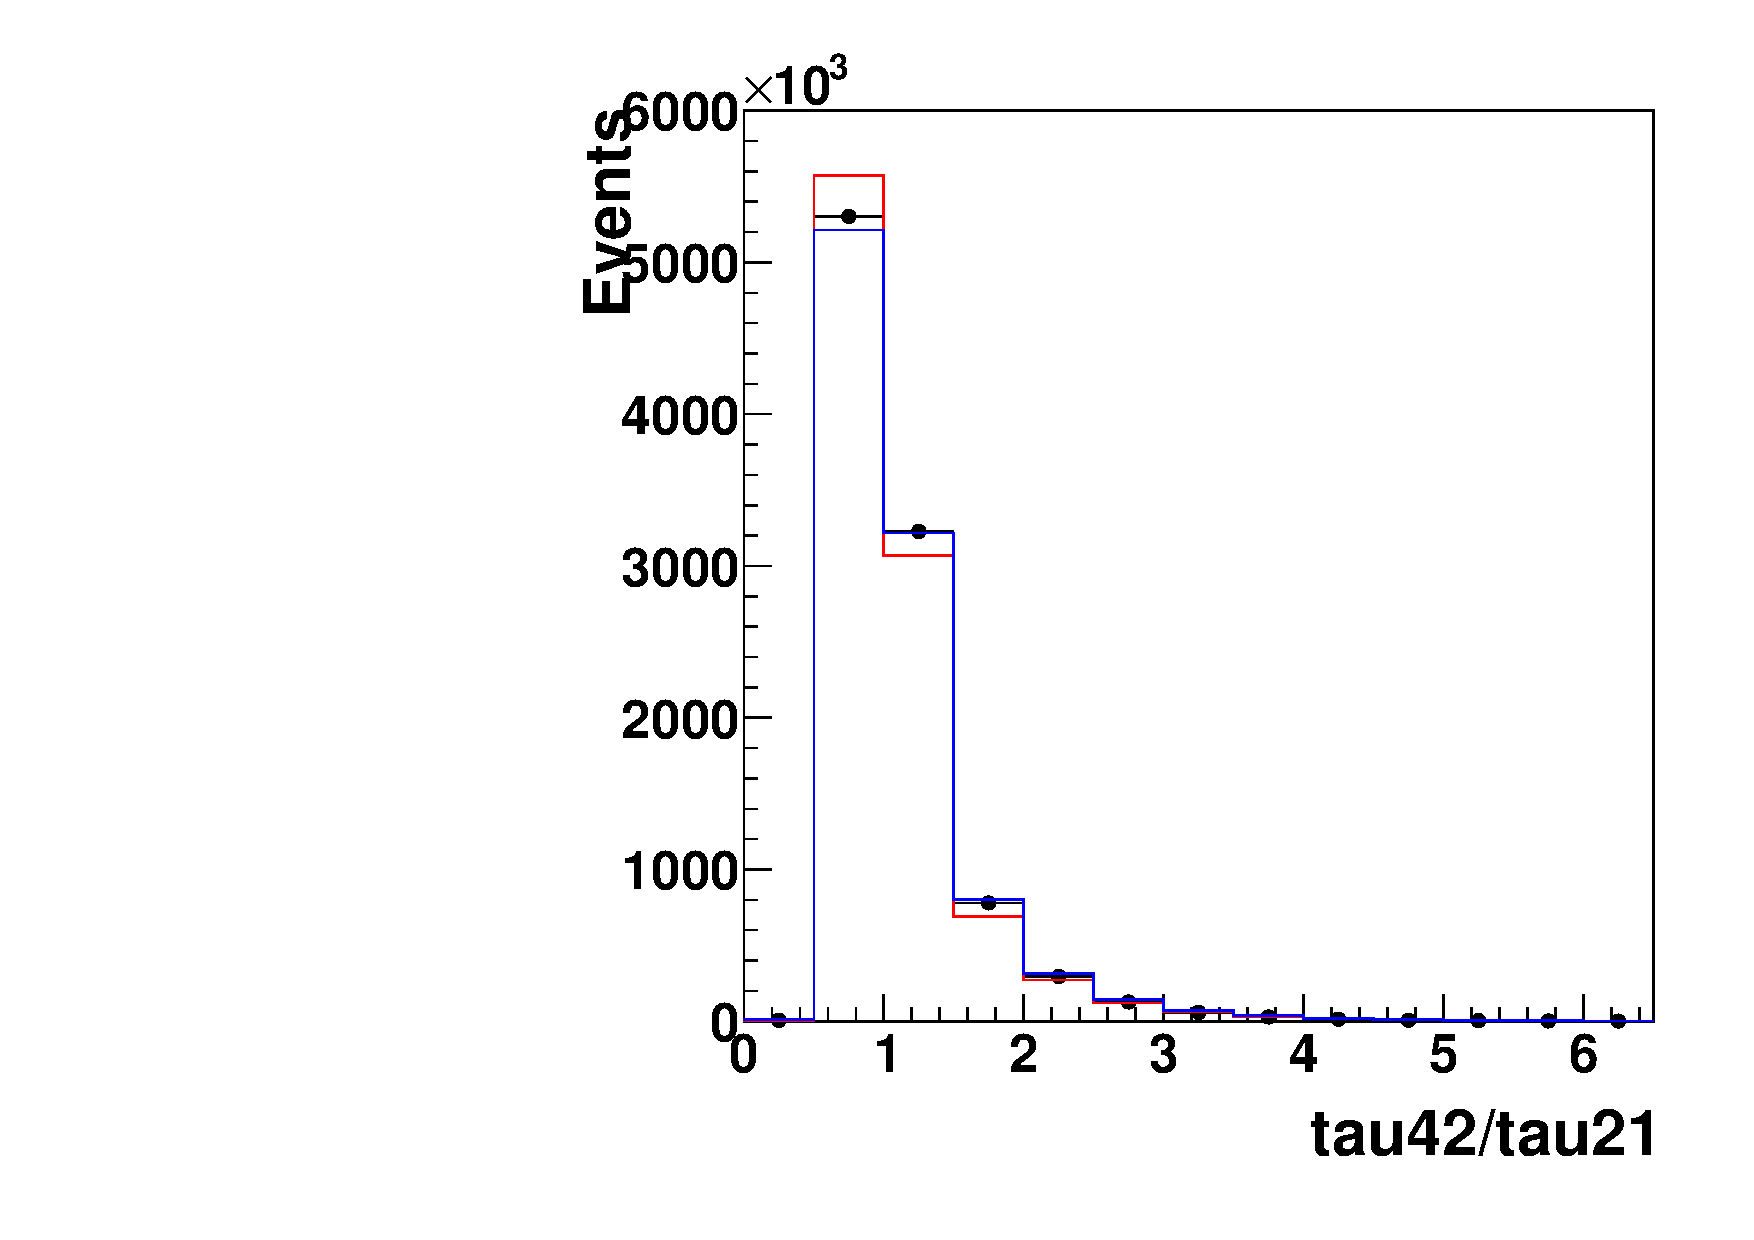
\includegraphics[width=0.49\textwidth,angle=0]{figs/SFExtra/SFSameJet.pdf}
\end{center}
\caption{
$\frac{\tau_{42}}{\tau_{21}}$ in data (black) compared to \PYTHIA QCD MC (red), and 
\HERWIG QCD MC (blue). Region of $0.55 < \tau_{42} < 0.65$ is shown. 
Left hand plot is logY scale. Plot on the right hand is corresponding 
ratio plot of left hand.  
}
\label{fig:tau4221samejetL}
\end{figure}

\clearpage
\newpage



Since Nsubjettiness $\tau_{N}$ is directly correlated with jet \pt, we further study
the $\frac{\tau_{42}}{\tau_{21}}$ with respect to the jet \pt, which are shown in 
Figure~\ref{fig:tau42212DPt}. 

\begin{figure}[ht!b]
\begin{center}
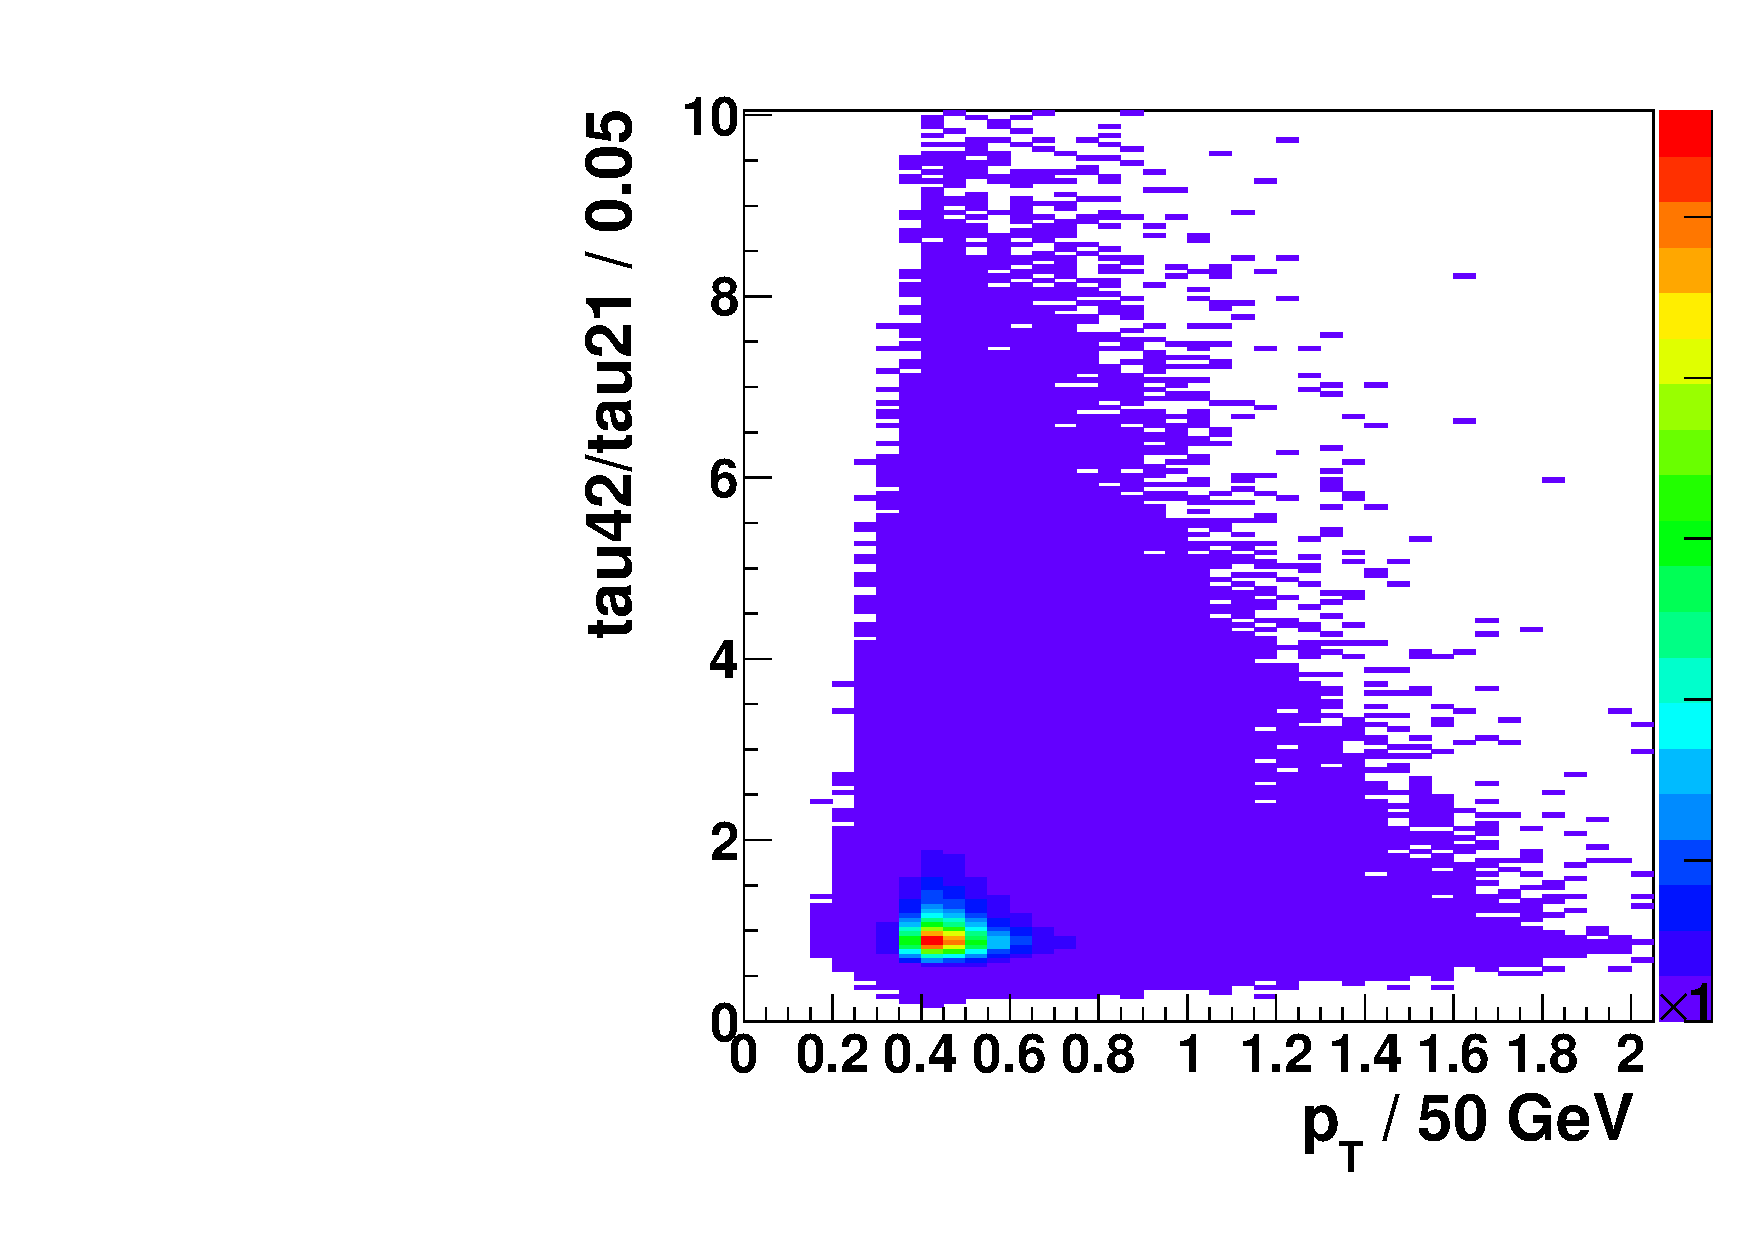
\includegraphics[width=0.6\textwidth,angle=0]{figs/SFExtra/tau4221Pt2DData.pdf}
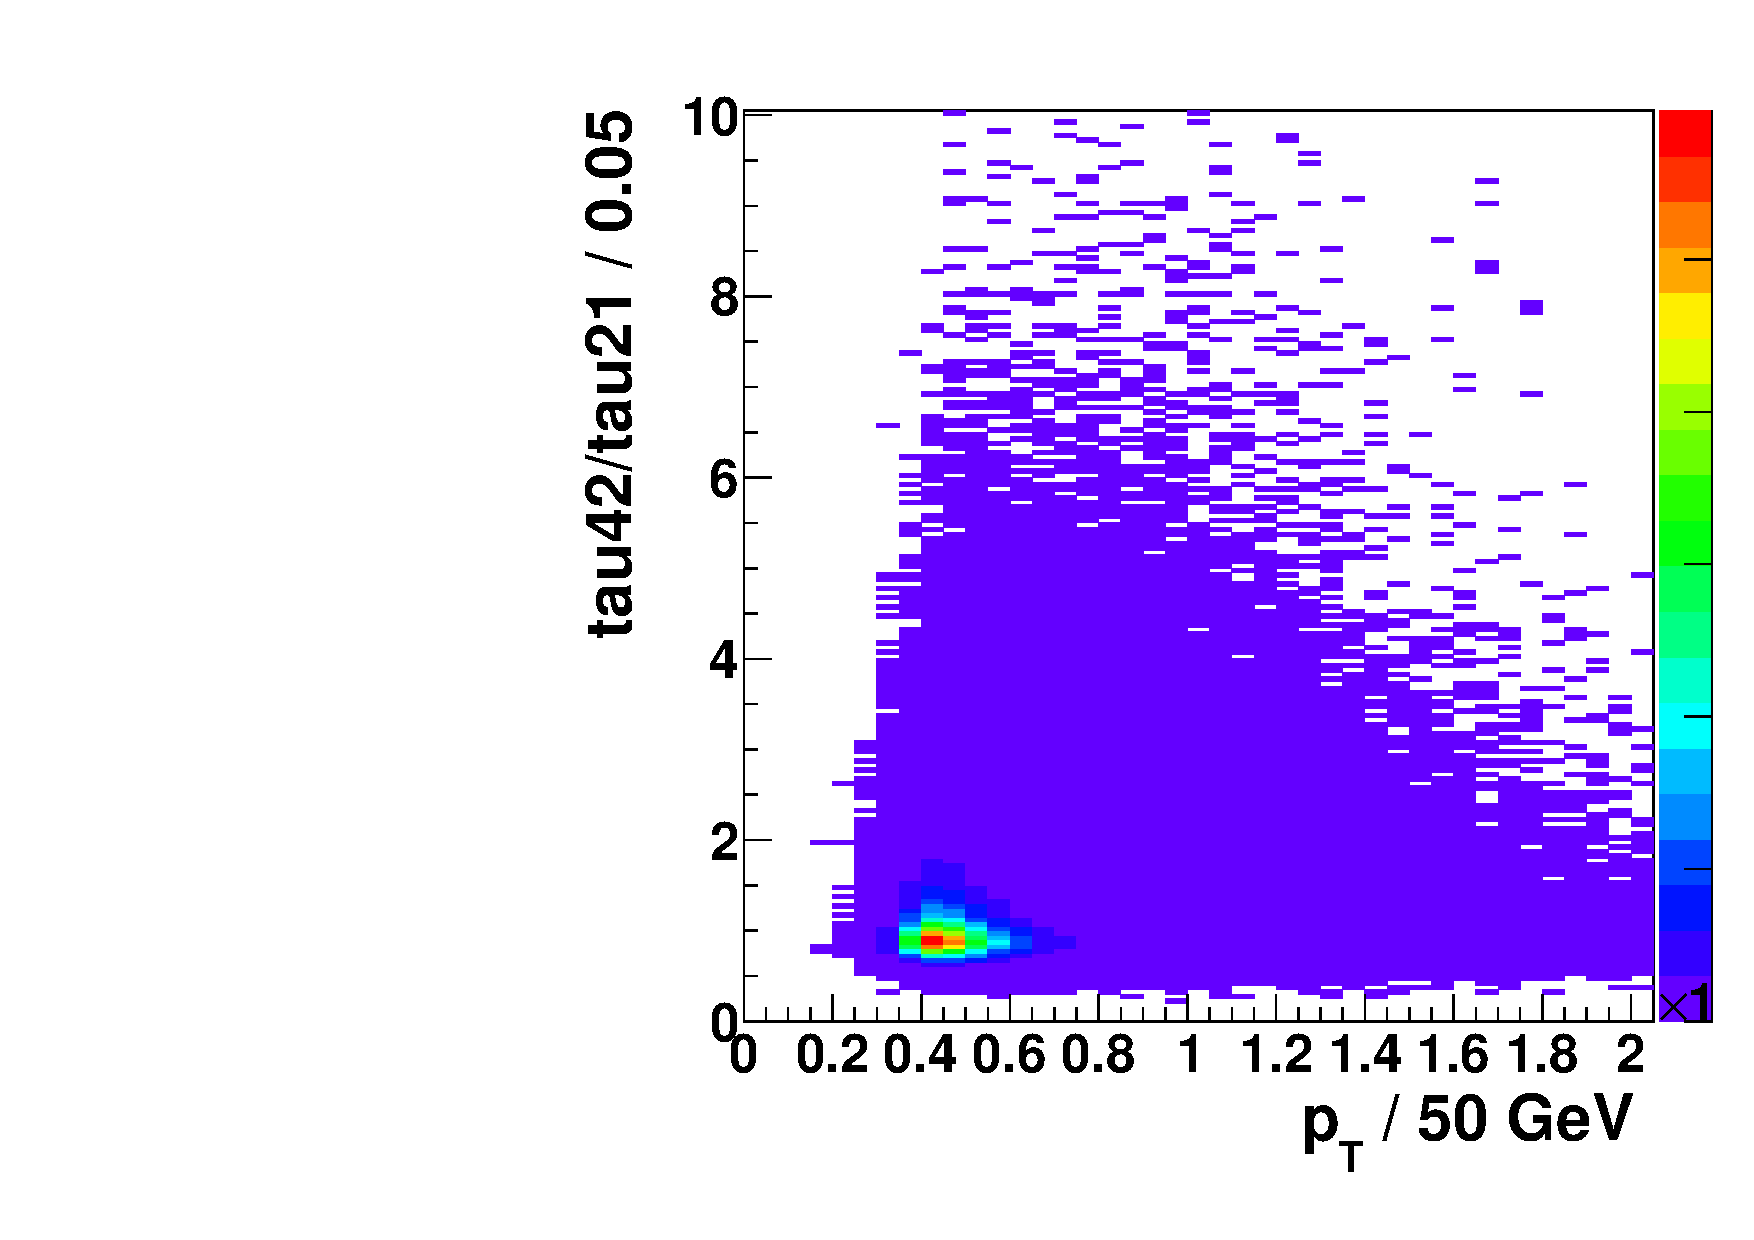
\includegraphics[width=0.49\textwidth,angle=0]{figs/SFExtra/tau4221Pt2DPythia.pdf}
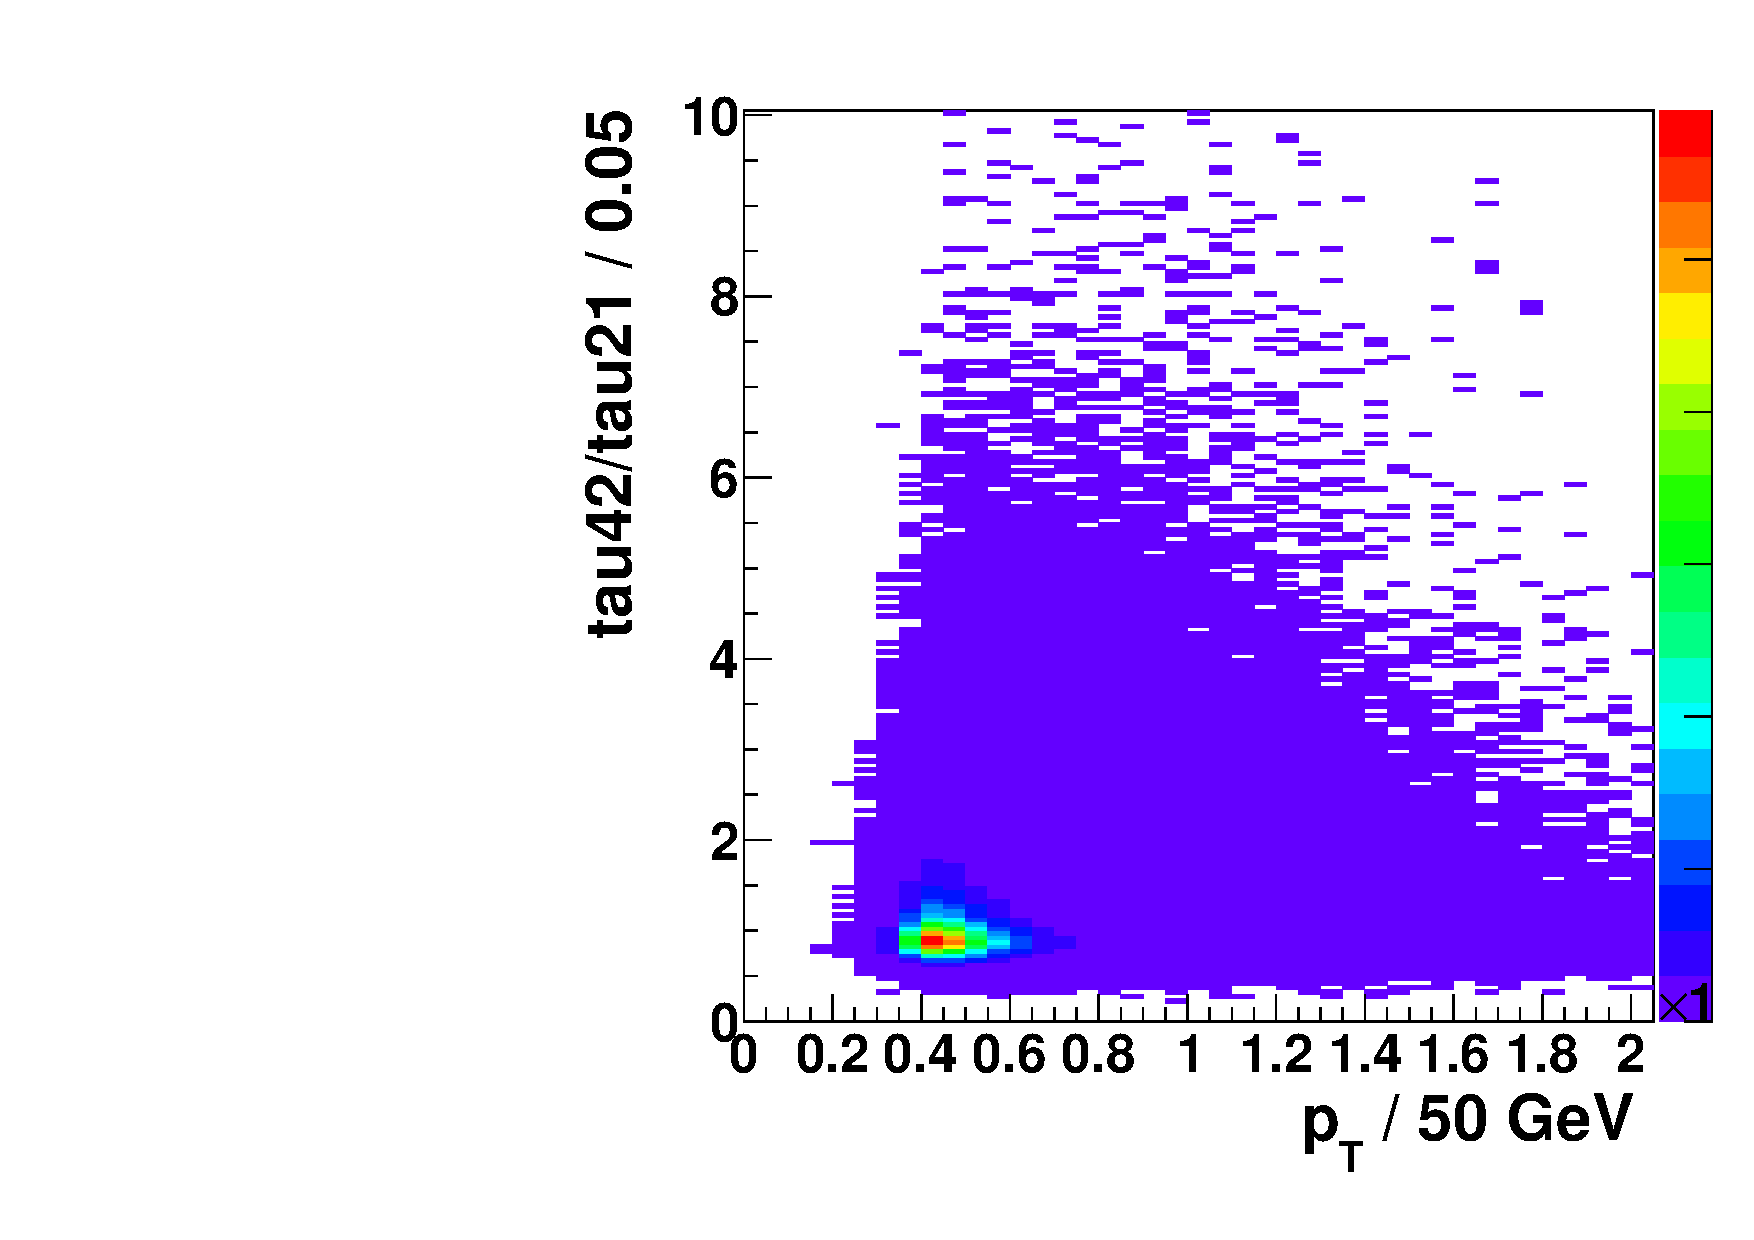
\includegraphics[width=0.49\textwidth,angle=0]{figs/SFExtra/tau4221Pt2DPythia.pdf}
\end{center}
\caption{ 2D Plot of
$\frac{\tau_{42}}{\tau_{21}}$ in Y axis, 
jet \pt in X axis, in data (top) compared to \PYTHIA QCD MC (bottom left), and
\HERWIG QCD MC (bottom right).
}
\label{fig:tau42212DPt}
\end{figure}

The corresponding profile plot of Figure~\ref{fig:tau42212DPt} is shown in 
Figure~\ref{fig:tau42212DPtProfile}. From this plot, QCD MC agrees well with 
data. However, they still have a small discrepancy respect to data, and also between
they seleves, especially at high \pt. To compensate this difference, we add an 
additional uncertainty $\epsilon$, as mentioned in the beginning of this section. 
$\epsilon$ represents the shower and hadronization difference of MC tools, i.e., 
\PYTHIA, \HERWIG.  We estimate $\epsilon$ by taking the largest difference in 
Higgs-tagging efficiency across various signal resonance masses, which results in 
7\%. 


\begin{figure}[htb]
\begin{center}
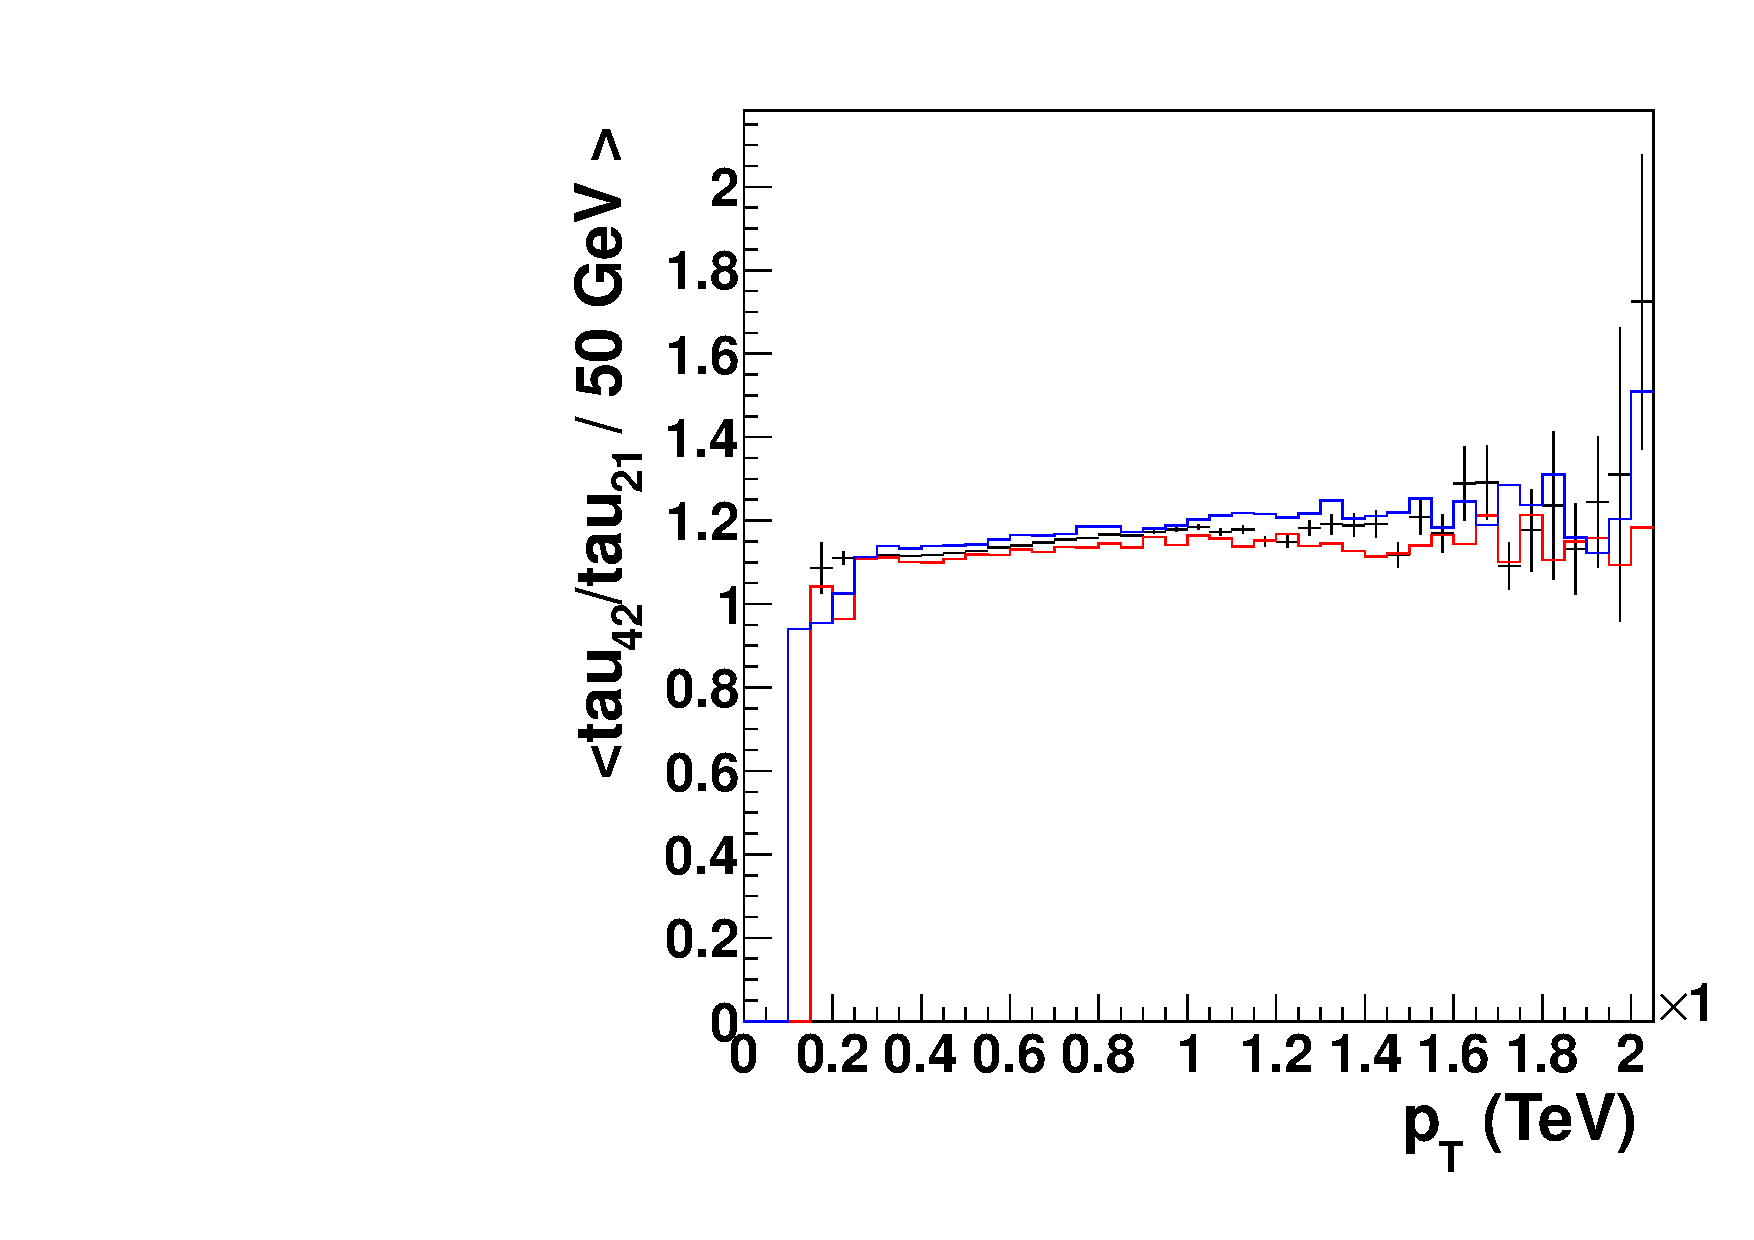
\includegraphics[width=0.6\textwidth,angle=0]{figs/SFExtra/tau4221PtProfile.pdf}
\end{center}
\caption{
Profile plot, mean of $\frac{\tau_{42}}{\tau_{21}}$ in Y axis, 
jet \pt in X axis, in data (black) compared to \PYTHIA QCD MC (red), and
\HERWIG QCD MC (blue).
}
\label{fig:tau42212DPtProfile}
\end{figure}


So the extrapolated scale factor for H-tagging is $0.86 \pm 7.6\% \pm 7.0\%$, 
for $\tau_{42} \leq  0.55$, while $1.39 \pm 54\% \pm 7.0\%$ for 
$0.55 < \tau_{42} <  0.65$.   


\clearpage


